\documentclass{article}
\usepackage{icml2026} 

\input{math_commands.tex}
\newcommand{\kT}{k_{\mathrm{T}}}
\usepackage{tikz}
\usetikzlibrary{shapes, arrows.meta, positioning, calc, fit, backgrounds, shadows.blur}

% Define colors for clarity
\definecolor{myblue}{RGB}{70, 130, 180}
\definecolor{myred}{RGB}{220, 20, 60}
\definecolor{mygreen}{RGB}{34, 139, 34}
\definecolor{myorange}{RGB}{255, 140, 0}
\usepackage{graphicx}

% Recommended packages for figures and better typesetting:
\usepackage{microtype}
\usepackage{graphicx}
\usepackage{makecell}
\usepackage{subcaption}
\usepackage{booktabs} % for professional tables
\newcommand{\pT}{p_{\mathrm{T}}}

% Use hyperref (hyperlinks in PDF)
\usepackage{hyperref}
\usepackage{xcolor} % for \definecolor
% Attempt to make hyperref and algorithmic work together better:
% \newcommand{\theHalgorithm}{\arabic{algorithm}}

% Use the following line for the initial blind version submitted for review:
\usepackage{icml2026}
% If accepted, instead use the following line for the camera-ready submission:
% \usepackage[accepted]{icml2026}

% Additional math packages
\usepackage{amsmath, amssymb, mathtools, amsthm}
% Cleveref if needed
\usepackage[capitalize,noabbrev]{cleveref}


\icmltitlerunning{Particle Hierarchical Attention Transformer for Jet Tagging}

\begin{document}

\twocolumn[
\icmltitle{Patch Attention Hierarchical Transformer for Efficient Particle Jet Tagging (PHAT-JeT)}


\begin{icmlauthorlist}
\icmlauthor{Aaron Wang}{equal,uic}
\icmlauthor{Zihan Zhao}{equal,ucsd}
\icmlauthor{Alan Xia}{equal, ucsd}
\icmlauthor{Abhijith Gandrakota}{fnal}
\icmlauthor{Jennifer Ngadiuba}{fnal}
\icmlauthor{Richard Cavanaugh}{uic}
\icmlauthor{Javier Duarte}{ucsd}
\end{icmlauthorlist}

\icmlaffiliation{uic}{University of Illinois Chicago, Chicago, IL 60607, USA}
\icmlaffiliation{ucsd}{University of California San Diego, La Jolla, CA 92093, USA}
\icmlaffiliation{fnal}{Fermi National Accelerator Laboratory, Batavia, IL 60510, USA}

\icmlcorrespondingauthor{Aaron Wang}{aaronw5@uic.edu}
\icmlcorrespondingauthor{Zihan Zhao}{ziz078@ucsd.edu}



\icmlkeywords{Machine Learning, ICML, Jet Tagging, Transformers, FPGA}

\vskip 0.3in
]
\printAffiliationsAndNotice{\icmlEqualContribution}

\begin{abstract}
Real-time jet tagging is critical for identifying short-lived particle decays in the high-throughput detectors of the Large Hadron Collider, where real-time trigger systems which are responsible for deciding which collision events to store impose strict latency and accuracy constraints.
While transformer models achieve strong performance in particle-level jet classification, their quadratic computational cost hinders deployment in strict real-time applications.
We introduce the \textbf{Patch Attention Hierarchical Transformer (PHAT-JeT)}, an attention-based model that incorporates a physics-inspired geometric message-passing module to encode local detector-plane structure prior to attention.
Global self-attention is replaced by a hierarchical patch-based mechanism that computes exact attention within small particle groups and preserves global context through a lightweight patch-token communication stage. 
For a fixed computational budget, PHAT-JeT achieves state-of-the-art accuracy and background rejection across multiple jet tagging benchmarks, outperforming existing models while remaining suitable for real-time deployment.
\end{abstract}




\section{Introduction}
\label{sec:intro}
At the Large Hadron Collider (LHC), protons traveling at nearly the speed of light collide 40 million times per second, producing enormous amounts of data~\cite{Evans:2008zzb}. These collisions recreate the extreme energy conditions of the early universe, producing unstable particles that existed microseconds after the Big Bang. Hidden within this torrent of familiar physics processes are extremely rare traces of new physics, and potential signatures of dark matter. Detecting these rare signals requires distinguishing them from overwhelming backgrounds in real time, a task that requires algorithms that are both extraordinarily fast and accurate~\cite{Deiana:2021niw,Harris:2022qtm}.

\begin{figure}[!ht]
\centering
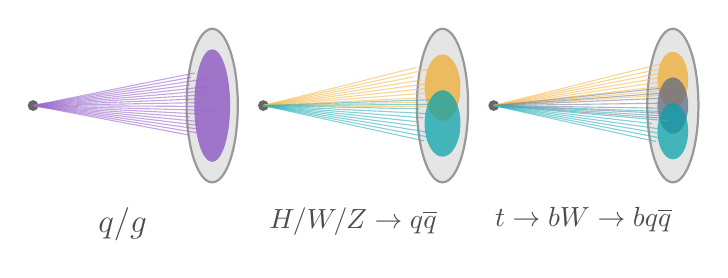
\begin{tikzpicture}[scale=0.65, every node/.style={scale=1.0}]

% --- NEW COLOR SCHEME ---
\definecolor{qgcolor}{RGB}{130, 70, 190}   % Purple (q/g jets)
\definecolor{ecal}{RGB}{0, 160, 170}       % Teal (EM deposits)
\definecolor{hcal}{RGB}{240, 170, 40}      % Amber/Gold (Hadronic deposits)
\definecolor{track}{RGB}{90, 100, 130}     % Slate Blue (Tracks)

% --- QUARK/GLUON JET (Left) ---
\begin{scope}[shift={(0,0)}]
    \fill[black!60] (0,0) circle (3pt);
    % Detector Circle with Grey Shade
    \draw[thick, black!40, fill=black!10] (3.5,0) ellipse (0.5cm and 1.5cm);
    
    % Single large blob (Purple)
    \fill[qgcolor, opacity=0.7] (3.5,0) ellipse (0.35cm and 1.1cm);
    
    \foreach \i in {1,...,18} {
        \pgfmathsetmacro{\angle}{-12 + \i*1.3} 
        \pgfmathsetmacro{\len}{3.3 + rand*0.3}
        \draw[qgcolor!80, thin, opacity=0.6] (0,0) -- (\angle:\len);
    }
    \node[below, black!70] at (1.75, -1.8) {\large $q/g$};
\end{scope}

% --- W/Z/HIGGS JET (Middle) ---
\begin{scope}[shift={(4.5,0)}]
    \fill[black!60] (0,0) circle (3pt);
    \draw[thick, black!40, fill=black!10] (3.5,0) ellipse (0.5cm and 1.5cm);
    
    % Upper prong (Amber)
    \fill[hcal, opacity=0.7] (3.5, 0.35) ellipse (0.35cm and 0.65cm);
    \foreach \i in {1,...,10} {
        \pgfmathsetmacro{\angle}{-2 + \i*1.6} 
        \pgfmathsetmacro{\len}{3.3 + rand*0.3}
        \draw[hcal!80, thin, opacity=0.6] (0,0) -- (\angle:\len);
    }
    
    % Lower prong (Teal)
    \fill[ecal, opacity=0.7] (3.5, -0.35) ellipse (0.35cm and 0.65cm);
    \foreach \i in {1,...,10} {
        \pgfmathsetmacro{\angle}{-14 + \i*1.6}
        \pgfmathsetmacro{\len}{3.3 + rand*0.3}
        \draw[ecal!80, thin, opacity=0.6] (0,0) -- (\angle:\len);
    }
    
    \node[below, black!70] at (1.75, -1.8) {$H/W/Z \to q\overline{q}$};
\end{scope}

% --- TOP QUARK JET (Right) ---
\begin{scope}[shift={(9.0,0)}]
    \fill[black!60] (0,0) circle (3pt);
    \draw[thick, black!40, fill=black!10] (3.5,0) ellipse (0.5cm and 1.5cm);
    
    % Top prong (Amber)
    \fill[hcal, opacity=0.7] (3.5, 0.5) ellipse (0.3cm and 0.55cm);
    \foreach \i in {1,...,8} {
        \pgfmathsetmacro{\angle}{2 + \i*1.5}
        \pgfmathsetmacro{\len}{3.3 + rand*0.2}
        \draw[hcal!80, thin, opacity=0.6] (0,0) -- (\angle:\len);
    }
    
    % Middle prong (Slate Blue)
    \fill[track, opacity=0.7] (3.5, 0.0) ellipse (0.3cm and 0.55cm);
    \foreach \i in {1,...,7} {
        \pgfmathsetmacro{\angle}{-6 + \i*1.7}
        \pgfmathsetmacro{\len}{3.4 + rand*0.2}
        \draw[track!80, thin, opacity=0.6] (0,0) -- (\angle:\len);
    }
    
    % Bottom prong (Teal)
    \fill[ecal, opacity=0.7] (3.5, -0.5) ellipse (0.3cm and 0.55cm);
    \foreach \i in {1,...,8} {
        \pgfmathsetmacro{\angle}{-14 + \i*1.5}
        \pgfmathsetmacro{\len}{3.3 + rand*0.2}
        \draw[ecal!80, thin, opacity=0.6] (0,0) -- (\angle:\len);
    }
    
    \node[below, black!70] at (1.75, -1.8) {$t \to bW \to bq\overline{q}$};
\end{scope}

\end{tikzpicture}
\caption{Schematic representation of jet substructures.
Left: Single-prong quark/gluon jet.
Middle: Two-prong boson decay ($H/W/Z$) with two subjets. 
Right: Three-prong top quark decay ($t$) with three subjets.}
\label{fig:jet_types}
\end{figure}

The challenge is formidable:
high-energy particle collisions at modern accelerators produce data at rates far beyond what can be permanently stored.
At the LHC, detectors generate raw data streams at the level of $\mathcal{O}(1~\mathrm{PB/s})$~\cite{Evans:2008zzb,CMSP2L1T}.
Since only a small fraction of these events can be recorded, real-time data filtering is performed by trigger systems that must decide, within $\mathcal{O}(10~\mu\mathrm{s})$, whether a collision event is potentially interesting for physics analyses~\cite{CMSL1T,ATLASL1T}.
The quality of these decisions directly determines which physical processes can be studied.

A central task for these real-time systems is jet tagging.
Many particles produced in high-energy collisions are quarks or gluons, which cannot be observed directly due to color confinement.
They instead hadronize into collimated sprays of particles that may be clustered into \emph{jets}~\cite{Cacciari:2008gp,Cacciari:2011ma}.
The internal structure of a jet encodes information about the underlying quark/gluon from which the jet originates and its decay history~\cite{Larkoski:2017jix}. 
Accurately identifying these patterns is essential for selecting rare signals and suppressing overwhelming background processes.
Even small improvements in tagging performance at the trigger level can translate into large gains in recorded signal yields and physics sensitivity, directly improving discovery potential for a global community of over ten thousand scientists.

Despite recent advances in jet-tagging performance, a substantial gap remains between models that achieve state-of-the-art accuracy and those that can be deployed in real-time trigger systems.
Highly expressive architectures such as the particle transformer~\cite{Qu2022} provide excellent discriminative power, but their large sizes and quadratic computational complexity make them impractical under strict latency and resource constraints.
Conversely, compact models that satisfy hardware requirements, such as small multilayer perceptrons (MLPs), lack sufficient representational capacity to distinguish complex jets.

This gap makes the development of well-performing, efficient ML architectures a critical requirement for trigger-level inference.
Such models must satisfy strict limits on latency, memory, and parameter count while maintaining sufficient expressive capacity to discriminate rare and complex physics signatures.
These requirements motivate the development of physics-inspired model architectures that explicitly encode relevant geometric and structural priors related to jet tagging, rather than relying on scaled-down versions of large, general-purpose networks~\cite{sanh2019distilbert, howard2017mobilenets, tan2019efficientnet}.
The core challenge is therefore to design models that are both efficient by construction and sufficiently expressive for jet tagging in real-time, hardware-limited environments.

To address this challenge, we propose the \textbf{Patch Hierarchical Attention Transformer for Jet Tagging (PHAT-JeT)}, which encodes physically meaningful structure through a geometric message-passing (GMP) module defined on a coarse grid to capture local energy flow patterns that are strongly correlated with the decay substructure of particles. 
Building on this geometry-aware representation, PHAT-JeT replaces global self-attention with a hierarchical, patch-based attention mechanism.
Fine-grained particle-particle interactions are computed within small patches, while a compact patch attention stage enables efficient global information exchange across the jet.
The patch size is a tunable hyperparameter that directly controls the computational cost, allowing the model to achieve near-linear scaling in the number of particles (tokens) while preserving expressive capacity. 
This design allows PHAT-JeT to exceed the performance of similar sized full-attention transformer models on jet tagging benchmarks. 
At the same time, its computational cost remains comparable to models currently deployed in trigger systems, making it practical for real-time deployment.

\section{Related Work}
A jet is naturally represented as an unordered set of particles with associated kinematic, particle-identification, and detector-related features, forming a point cloud in momentum space.
This formulation connects jet tagging to the broader class of point-cloud and set learning problems, where permutation-equivariant architectures and geometric deep learning have proven effective at capturing local structure and global correlations~\cite{qi2017pointnetdeeplearningpoint,ds}.
However, general-purpose point-cloud models are not designed for the extreme latency and resource constraints imposed by real-time trigger systems.
Existing efficient transformer-style models for point clouds and jet tagging often rely on explicit sparsification, strong locality assumptions, or particle serialization to reduce computational cost~\cite{wu2024pointtransformerv3simpler}.
In particular, many recent point-cloud transformers achieve scalability by imposing an ordering on the input through spatial serialization or sorting, which introduces a sequential dependency that limits parallelism and complicates deployment on low-latency hardware.

Early jet-tagging methods relied on hand-engineered observables combined with multivariate classifiers or image-based representations processed with convolutional neural networks. 
While computationally efficient, these approaches depend on fixed feature representations and struggle to capture the full relational structure of jet constituents.
More recent methods treat a jet as an unordered set of particles, enabling permutation-invariant architectures by construction. Set-based models such as deep sets~\cite{ds} and energy flow networks~\cite{efn} provide simple and efficient baselines, but their global aggregation fundamentally limits their ability to model complex, multi-scale correlations.

Geometric deep learning approaches explicitly model particle-particle relationships. Interaction networks~\cite{NIPS2016_3147da8a} inspired graph-based jet taggers such as JEDI-net~\cite{jedi}, which learn relational features between all particle pairs. ParticleNet adapts the dynamical graph convolutional neural network~\cite{dgcnn} by constructing local neighborhoods and learning hierarchical geometric features~\cite{Qu:2019gqs}. 
Although these methods achieve strong performance, their reliance on pairwise or neighborhood-based message passing introduces significant computational overhead, making them difficult to deploy under strict real-time constraints.

Transformers have become the most accurate class of models for jet tagging because self-attention can capture rich global correlations among all constituents.
Particle transformer applies full self-attention to particle clouds and achieves state-of-the-art jet tagging results~\cite{Qu2022}.
Subsequent work has analyzed attention structure and sparsity and explored acceleration strategies~\cite{Wang:2024rup,legge2025attentionsparseparticletransformer}.
Symmetry-aware variants, including Lorentz group attention transformers and Lorentz-equivariant models based on geometric algebra, incorporate relativistic structure directly into the attention mechanism~\cite{spinner2024lorentzequivariantgeometricalgebratransformers}.
Despite their expressivity, all of these approaches scale quadratically with the number of particles, leading to prohibitive latency and memory usage in real-time, hardware-limited environments.

A parallel line of work focuses on reducing the cost of attention.
General-purpose methods such as Linformer approximate attention with low-rank projections~\cite{wang2020linformer}.
JEDI-linear replaces nonlinear message passing with linear aggregation to enable fast FPGA inference, but this simplification limits representational power~\cite{que2025jedilinearfastefficientgraph}.
Some models incorporate particle physics inductive biases into model design, such as SAL-T, which restricts attention to spatially local groups and injects geometry through lightweight convolutions, reducing cost at the expense of global context~\cite{wang2025spatiallyawarelineartransformer}. 

In prior work on ultra-low-latency jet tagging, there remains a gap between models that capture rich global context and models that meet strict hardware constraints.
Existing approaches often either treat jets as unstructured sets, limiting hierarchical reasoning, or rely heavily on local receptive fields that weaken long-range correlations.
A more physics-driven design should exploit the inherently hierarchical organization of hadronic showers to enable efficient, multi-scale attention.
To this end, we introduce PHAT-JeT, an attention-based architecture for particle-cloud jet tagging under ultra-low-latency constraints.



\section{PHAT-JeT}

\subsection*{Geometric Message Passing}
The substructure of a jet is defined by the angular distribution of its constituents in the detector.
Each particle is characterized by its transverse momentum $\pT$ and its angular coordinates $(\eta,\phi)$, where $\eta$ is the pseudorapidity and $\phi$ is the azimuthal angle around the beam axis.
Decays of target rare heavy particles produce characteristic multi-prong energy deposits within a single jet cone, which appear as localized clusters in the $(\eta,\phi)$ plane. Accurately capturing these angular correlations and transverse energy flow patterns is therefore essential for jet tagging.
While transformer models are permutation-equivariant, they require an explicit notion of position to distinguish between particles.
For jets, this notion of position is naturally geometric and is given by the relative locations of particles in the $(\eta,\phi)$ plane. 

We therefore introduce a learned \emph{geometric message-passing}  module that injects local angular context into the particle embeddings using a lightweight 2D convolution over a coarse detector grid.
\begin{figure}[!ht]
\centering
\resizebox{\columnwidth}{!}{%
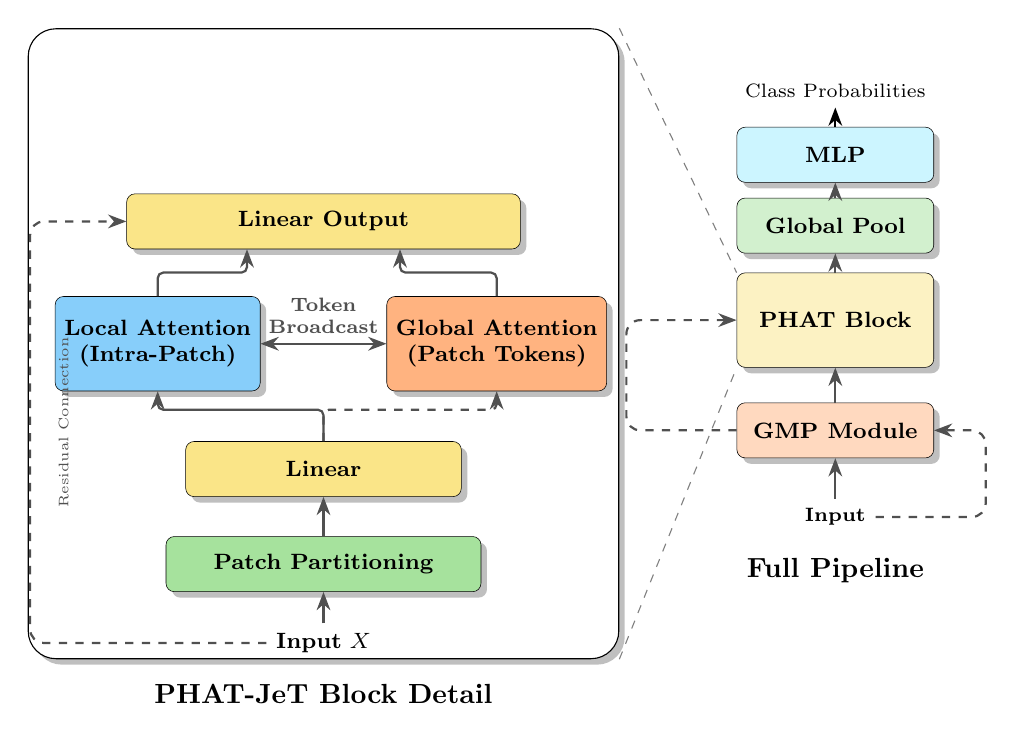
\begin{tikzpicture}[
    font=\sffamily\bfseries,
    >=Stealth,
    node distance=0.5cm,
    % Define colors
    /utils/exec={
        \definecolor{phatYellow}{RGB}{250, 229, 136}
        \definecolor{phatCyan}{RGB}{153, 235, 255}
        \definecolor{phatBlue}{RGB}{135, 206, 250}
        \definecolor{phatGreen}{RGB}{166, 226, 157}
        \definecolor{phatOrange}{RGB}{255, 179, 128}
        \definecolor{phatGrey}{RGB}{245, 245, 245}
        \definecolor{phatDarkGrey}{RGB}{80, 80, 80}
    },
    % Node Styles
    block/.style={
        draw=black, very thin, rounded corners=3pt, 
        minimum height=0.7cm, minimum width=1.8cm, 
        align=center, font=\footnotesize\bfseries, drop shadow
    },
    linear/.style={block, fill=phatYellow},
    attn/.style={block, fill=phatBlue, minimum height=1.2cm, minimum width=2.2cm},
    global_attn/.style={block, fill=phatOrange, minimum height=1.2cm, minimum width=2.2cm},
    patch/.style={block, fill=phatGreen, minimum width=4cm},
    container/.style={
        draw=black, fill=phatGrey, rounded corners=10pt, 
        inner sep=0.3cm, drop shadow
    },
    conn/.style={->, thick, phatDarkGrey, rounded corners=2pt},
    res_conn/.style={->, thick, phatDarkGrey, dashed, rounded corners=5pt}
]

% =================================================================
% LEFT SIDE: MICRO VIEW (Single Linear Box)
% =================================================================

% --- Main Container ---
\node[container, minimum width=7.5cm, minimum height=8.0cm, fill=white] (mainBox) at (0, 3.5) {};

% --- INPUT ---
\node[font=\footnotesize] (inputNode) at (0, -0.3) {\textbf{Input} $X$};

% --- PATCHING (First) ---
\node[patch, above=0.4cm of inputNode] (patching) {Patch Partitioning};
\draw[conn] (inputNode) -- (patching);

% --- LINEAR LAYER (Merged) ---
% Replaced 3 Q/K/V boxes with one single Linear box
\node[linear, above=0.5cm of patching, minimum width=3.5cm] (linProj) {Linear};

% Connect Patching to Linear
\draw[conn] (patching) -- (linProj);

% --- ATTENTION MODULES ---
\coordinate (attnCenter) at (0, 3.5);

% Attention blocks separated by gap
\node[attn, anchor=east] (localAttn) at ($(attnCenter) + (-0.8, 0)$) {Local Attention\\(Intra-Patch)};
\node[global_attn, anchor=west] (globalAttn) at ($(attnCenter) + (0.8, 0)$) {Global Attention\\(Patch Tokens)};

% Connections from Single Linear to Attention
% Solid line to Local Attention
\draw[conn] (linProj.north) -- ++(0, 0.4) -| (localAttn.270);
% Dashed line to Global Attention
\draw[conn, dashed] (linProj.north) -- ++(0, 0.4) -| (globalAttn.270);

% Exchange Arrow
\draw[<->, thick, phatDarkGrey] (localAttn) -- node[above, font=\scriptsize\bfseries, align=center, midway] {Token\\Broadcast} (globalAttn);

% --- OUTPUT STAGE ---
\node[linear, above=1.2cm of attnCenter, minimum width=5cm] (linOut) {Linear Output};

% Merge Connections
\draw[conn] (localAttn.north) -- ++(0, 0.3) -| (linOut.200);
\draw[conn] (globalAttn.north) -- ++(0, 0.3) -| (linOut.340);

% RESIDUAL CONNECTION
\draw[res_conn] (inputNode.west) -- ++(-3.0, 0) |- (linOut.west);
\node[font=\tiny, rotate=90, color=phatDarkGrey] at (-3.3, 2.5) {Residual Connection};

\node[below=0.2cm of mainBox.south, font=\bfseries] {PHAT-JeT Block Detail};


% =================================================================
% RIGHT SIDE: MACRO VIEW (Unchanged)
% =================================================================
\begin{scope}[shift={(6.5, 1.5)}]

    % Input
    \node[font=\bfseries\scriptsize] (x_in) at (0, -0.2) {Input};

    % GMP
    \node[block, fill=phatOrange!50, minimum width=2.5cm] (gmp_layer) at (0, 0.9) {GMP Module};
    
    % PHAT BLOCK
    \node[block, fill=phatYellow!50, minimum width=2.5cm, minimum height=1.2cm] (phat_block) at (0, 2.3) {PHAT Block};

    % Global Pool
    \node[block, fill=phatGreen!50, minimum width=2.5cm] (pool) at (0, 3.5) {Global Pool};

    % MLP
    \node[block, fill=phatCyan!50, minimum width=2.5cm] (mlp) at (0, 4.4) {MLP};
    
    % Output
    \draw[->, thick] (mlp) -- ++(0, 0.6) node[above, font=\scriptsize] {Class Probabilities};

    % Connections
    \draw[conn] (x_in) -- (gmp_layer);
    \draw[conn] (gmp_layer) -- (phat_block);
    \draw[conn] (phat_block) -- (pool);
    \draw[conn] (pool) -- (mlp);
    
    % Residual 1
    \draw[res_conn] (x_in.east) -- ++(1.4, 0) |- (gmp_layer.east);

    % Residual 2
    \draw[res_conn] (gmp_layer.west) -- ++(-1.4, 0) |- (phat_block.west);

    % Zoom Lines
    \draw[gray, thin, dashed] (mainBox.north east) -- (phat_block.north west);
    \draw[gray, thin, dashed] (mainBox.south east) -- (phat_block.south west);

    \node[below=2.3cm of phat_block, font=\bfseries] {Full Pipeline};

\end{scope}

\end{tikzpicture}%
}
\caption{Architecture of PHAT-JeT. (Left) The PHAT block partitions input particles into patches before projection. (Right) The full pipeline includes geometric message passing (GMP) prior to the attention block.}
\label{fig:phat_arch_patchfirst}
\end{figure}
Let $X \in \mathbb{R}^{N\times C}$ denote the particle embeddings for a single jet, with coordinates $(\eta_i,\phi_i)$. We quantize each particle to a detector grid of spacing $\delta$ using per-jet minimum shifts
\begin{equation}
u_i = \left\lfloor \frac{\eta_i - \eta_{\min}}{\delta} \right\rfloor,
\qquad
v_i = \left\lfloor \frac{\phi_i - \phi_{\min}}{\delta} \right\rfloor,
\end{equation}
where $\eta_{\min}=\min_j \eta_j$ and $\phi_{\min}=\min_j \phi_j$ ensure nonnegative indices.

We construct a 2D feature map by summing particle features within each grid cell
\begin{equation}
G_{u,v} = \sum_{i:(u_i,v_i)=(u,v)} X_i ,
\end{equation}
yielding $G \in \mathbb{R}^{H\times W\times C}$ for appropriate grid dimensions $(H,W)$.
A depthwise 2D convolution is applied to the grid representation
\begin{equation}
\tilde{G} = \mathrm{DWConv}(G).
\end{equation}

We then sample the convolved grid back at the particle locations
\begin{equation}
Z_i = \tilde{G}_{u_i,v_i},
\end{equation}
and apply a pointwise channel mixing (shared across particles)
\begin{equation}
Y_i = W_p Z_i ,
\end{equation}
where $W_p \in \mathbb{R}^{C\times C}$ is a learned linear projection.

Finally, the positional features are normalized and added residually to the input embeddings.

The GMP can be interpreted as applying a small learnable spatial filter to a coarse, image-like representation of the jet in the $(\eta,\phi)$ plane.
Each grid cell aggregates the features of particles that fall within the same angular region, forming a low-resolution map of the jet's energy and feature distribution.
The convolution then propagates information between neighboring angular regions, allowing each particle to incorporate context from its surrounding area in the detector.
In this way, GMP encodes local geometric structure and correlations that reflect the underlying decay topology, while remaining invariant to particle ordering and computationally inexpensive.
This design aligns naturally with the detector geometry and provides a physically meaningful positional encoding for subsequent attention layers.

The role of the GMP module is precisely to inject local angular structure before attention, such that subsequent patch interactions operate on geometry-aware embeddings rather than raw kinematic coordinates.
%========================================================

\begin{figure*}[!ht]
\centering
% \resizebox{\textwidth}{!}{%
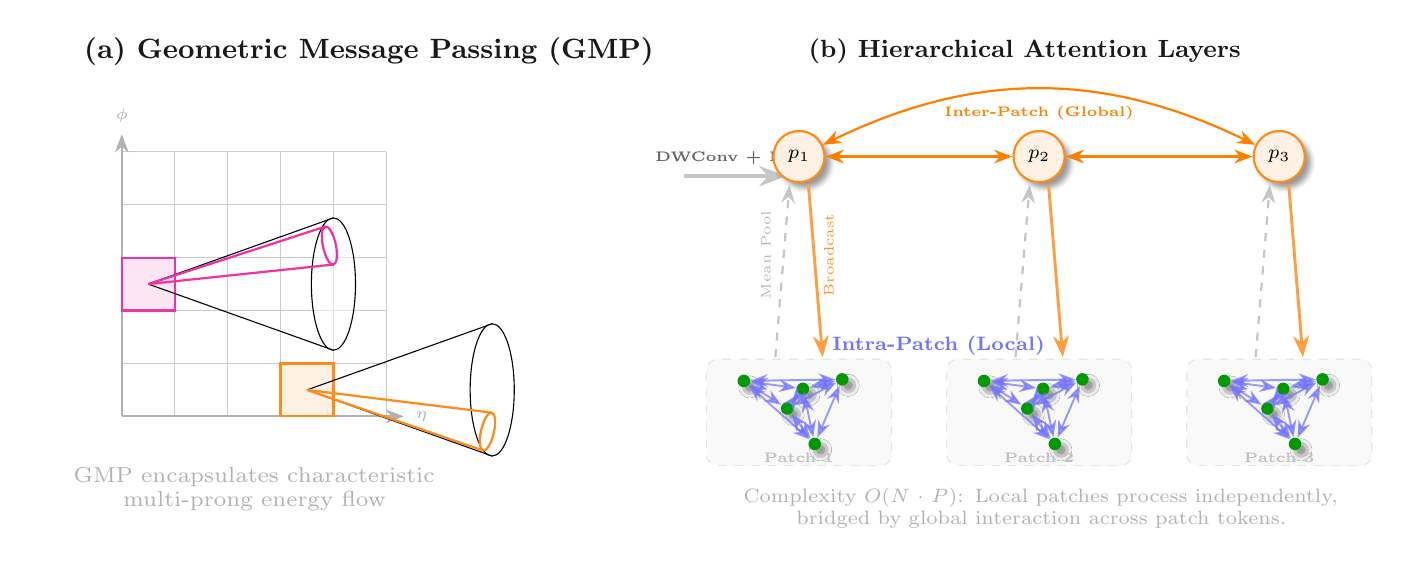
\begin{tikzpicture}[
    font=\sffamily,
    >=Stealth,
    % ---------------- Styles ----------------
    particle/.style={circle, fill=blue!60!cyan, inner sep=1.4pt, blur shadow={shadow blur steps=2}},
    enhanced_particle/.style={particle, fill=green!60!black, inner sep=1.6pt},
    gridcell/.style={draw=gray!30, fill=white, thin},
    activecell/.style={draw=orange, thick, fill=orange!16},
    patchbox/.style={rounded corners=4pt, draw=gray!20, fill=gray!5, dashed},
    token/.style={circle, draw=orange!90, fill=orange!10, thick, inner sep=2pt, minimum size=0.65cm,
                  font=\scriptsize\bfseries, blur shadow},
    section_label/.style={font=\small\bfseries, color=black!90},
    flow_arrow/.style={->, line width=1.5pt, color=gray!45},
    local_attn/.style={blue!55, line width=0.7pt, opacity=0.70},
    local_attn_arrow/.style={local_attn, <->},
    % --- GMP STYLES ---
    cellPink/.style={draw=magenta!80, fill=magenta!10, thick},
    cellOrange/.style={draw=orange!90, fill=orange!10, thick},
    jetBlack/.style={draw=black, thin, fill=gray!5, opacity=0.8},
    subjetPink/.style={draw=magenta!80, thick, fill=magenta!20},
    subjetOrange/.style={draw=orange!90, thick, fill=orange!20},
    gridLine/.style={gray!40, thin}
]

% ==========================================================================================
% (A) GEOMETRIC MESSAGE PASSING (GMP)
% ==========================================================================================
\begin{scope}[local bounding box=gmp, scale=1.12, transform shape]
    \node[section_label, anchor=south west] at (-0.55, 3.85) {(a) Geometric Message Passing (GMP)};

    % Discretized grid (5x5, size 3.0, step 0.6)
    \draw[gridLine] (0,0) grid[step=0.6] (3.0, 3.0);

    % Axes
    \draw[->, gray!60, thick] (0,0) -- (3.2,0) node[right, font=\tiny] {$\eta$};
    \draw[->, gray!60, thick] (0,0) -- (0,3.2) node[above, font=\tiny] {$\phi$};

    % --- CELL 1 (Pink) at (1, 3) ---
    % Grid: 5x5. Col 1 is x=0.0-0.6. Row 3 is y=1.2-1.8 (Vertical Center)
    \draw[cellPink] (0.0, 1.2) rectangle (0.6, 1.8);
    \coordinate (c1) at (0.3, 1.5); 

    % --- CELL 2 (Orange) at (4, 1) ---
    % Grid: 5x5. Col 4 is x=1.8-2.4. Row 1 is y=0.0-0.6 (Bottom)
    \draw[cellOrange] (1.8, 0.0) rectangle (2.4, 0.6);
    \coordinate (c2) at (2.1, 0.3); 

    % --- CONE 1 (Pink) ---
    % Position: Middle Row (y=1.5) -> Angle 0
    \begin{scope}[shift={(c1)}]
        \def\coneL{2.1} \def\coneR{0.75} \def\subR{0.22} \def\persp{0.25}
        % Outer Cone
        \draw[black, thin] (0,0) -- (\coneL, \coneR);
        \draw[black, thin] (0,0) -- (\coneL, -\coneR);
        \draw[black, thin, fill=white, fill opacity=0.5] (\coneL, 0) ellipse ({\persp} and \coneR);
        
        % Inner Subjet (Angle 0)
        \begin{scope}[rotate=12]
            \pgfmathsetmacro{\subPersp}{(\subR/\coneR)*\persp}
            \draw[subjetPink, fill opacity=0.5] (0,0) -- (\coneL, \subR);
            \draw[subjetPink, fill opacity=0.5] (0,0) -- (\coneL, -\subR);
            \draw[subjetPink, fill=white] (\coneL, 0) ellipse ({\subPersp} and \subR);
        \end{scope}
    \end{scope}

    % --- CONE 2 (Orange) ---
    % Position: Bottom Row (y=0.3) -> Angle -20
    \begin{scope}[shift={(c2)}]
        \def\coneL{2.1} \def\coneR{0.75} \def\subR{0.22} \def\persp{0.25}
        % Outer Cone
        \draw[black, thin] (0,0) -- (\coneL, \coneR);
        \draw[black, thin] (0,0) -- (\coneL, -\coneR);
        \draw[black, thin, fill=white, fill opacity=0.5] (\coneL, 0) ellipse ({\persp} and \coneR);
        
        % Inner Subjet (Angle -20)
        \begin{scope}[rotate=-13]
            \pgfmathsetmacro{\subPersp}{(\subR/\coneR)*\persp}
            \draw[subjetOrange, fill opacity=0.5] (0,0) -- (\coneL, \subR);
            \draw[subjetOrange, fill opacity=0.5] (0,0) -- (\coneL, -\subR);
            \draw[subjetOrange, fill=white] (\coneL, 0) ellipse ({\subPersp} and \subR);
        \end{scope}
    \end{scope}

    % Labels

    \node[anchor=north, font=\scriptsize, align=center, text width=4.9cm, color=gray!60] at (1.5, -0.45)
        {GMP encapsulates characteristic\\ multi-prong energy flow};
\end{scope}

% ==========================================================================================
% FLOW ARROW
% ==========================================================================================
\draw[flow_arrow] ($(gmp.east) + (0.25, 1.25)$) -- ($(gmp.east) + (1.55, 1.25)$)
    node[midway, above, font=\tiny\bfseries, color=black!60] {DWConv + MLP};

% =============================================% ==========================================================================================
% (B) HIERARCHICAL ATTENTION: further overlap fixes
%  - move all left-side labels INSIDE the panel and away from incoming DWConv arrow
%  - move "Inter-Patch (Global)" above token row (not on same y as p1)
%  - move "Intra-Patch (Local)" above patch row (left, no overlap)
%  - move Mean Pool/Broadcast labels between p1 and patch1 (not over arrows)
% ==========================================================================================
\begin{scope}[shift={(8.6, 0)}, local bounding box=attn]
    \node[section_label, anchor=south west] at (0, 4.35) {(b) Hierarchical Attention Layers};

    % --- spacing knobs ---
    \def\tokY{3.30}        % token row y
    \def\patchY{0.05}      % patch block baseline y
    \def\dx{3.05}          % horizontal spacing
    \def\labXin{0.05}      % left labels x (INSIDE panel)

    % Tokens
    \node[token] (t1) at (0.0, \tokY) {$p_1$};
    \node[token] (t2) at (\dx, \tokY) {$p_2$};
    \node[token] (t3) at (2*\dx, \tokY) {$p_3$};

    % Global links
    \draw[<->, orange, thick] (t1) -- (t2);
    \draw[<->, orange, thick] (t2) -- (t3);
    \draw[<->, orange, thick, bend left=26] (t1) to (t3);

    % Global label: put it HIGHER so it doesn't sit on arrows
    \node[font=\tiny\bfseries, color=orange] at ($(t1)!0.5!(t3) + (0,0.55)$)
        {Inter-Patch (Global)};

    % -------------------- Intra-patch label (move ABOVE patch row, left)
    \node[anchor=west, font=\scriptsize\bfseries, color=blue!55]
        at (\labXin+0.25, \patchY+0.85) {Intra-Patch (Local)};

    % Patch boxes + particles
    \foreach \x/\idx in {0/1, \dx/2, {2*\dx}/3} {
        \begin{scope}[shift={(\x, \patchY)}]
            \node[patchbox, minimum width=2.35cm, minimum height=1.35cm] (pb\idx) {};

            \node[enhanced_particle] (p\idx a) at (-0.70, 0.40) {};
            \node[enhanced_particle] (p\idx b) at ( 0.55, 0.42) {};
            \node[enhanced_particle] (p\idx c) at ( 0.20,-0.40) {};
            \node[enhanced_particle] (p\idx d) at (-0.15, 0.05) {};
            \node[enhanced_particle] (p\idx e) at ( 0.05, 0.30) {};

            \draw[local_attn_arrow] (p\idx a)--(p\idx b);
            \draw[local_attn_arrow] (p\idx a)--(p\idx c);
            \draw[local_attn_arrow] (p\idx a)--(p\idx d);
            \draw[local_attn_arrow] (p\idx a)--(p\idx e);
            \draw[local_attn_arrow] (p\idx b)--(p\idx c);
            \draw[local_attn_arrow] (p\idx b)--(p\idx d);
            \draw[local_attn_arrow] (p\idx b)--(p\idx e);
            \draw[local_attn_arrow] (p\idx c)--(p\idx d);
            \draw[local_attn_arrow] (p\idx c)--(p\idx e);
            \draw[local_attn_arrow] (p\idx d)--(p\idx e);

            \node[font=\tiny\bfseries, gray!50, anchor=south]
                at ($(pb\idx.south)+(0,-0.08)$) {Patch \idx};
        \end{scope}
    }

    % Pooling + broadcast arrows (same geometry, but cleaner)
    \foreach \tok/\pb in {t1/pb1, t2/pb2, t3/pb3} {
    % mean pool (dashed up)
    \draw[->, dashed, color=gray!45, thick]
        ($(\pb.north) + (-0.30, 0.02)$) -- ($(\tok.south) + (-0.12, -0.02)$);
    % broadcast (solid down)
    \draw[->, solid, color=orange!75, line width=1.05pt]
        ($(\tok.south) + (0.12, -0.02)$) -- ($(\pb.north) + (0.30, 0.02)$);
}

    % Put Mean Pool / Broadcast labels BETWEEN t1 and pb1, not on the left margin
    \node[font=\tiny, color=gray!55, rotate=90]   at (-0.42, 2.05) {Mean Pool};
    \node[font=\tiny, color=orange!85, rotate=90] at ( 0.38, 2.05) {Broadcast};

    % Bottom caption
    \node[anchor=north, font=\scriptsize, align=center, text width=8.6cm, color=gray!60]
        at (\dx, -0.78)
        {Complexity $O(N \cdot P)$: Local patches process independently,\\
         bridged by global interaction across patch tokens.};
\end{scope}
\end{tikzpicture}%
% } 
\caption{Particle Hierarchical Attention Transformer (PHAT) schematic. (a) GMP discretizes the $(\eta,\phi)$ plane and mixes nearby cells, capturing multi-prong substructure. (b) Exact local attention within patches and lightweight global interaction via patch tokens.}
\label{fig:phat_schematic}
\end{figure*}

\subsection*{Local Patch-Based Self-Attention}
\label{subsec:local_patch_attention}
To make attention tractable under strict latency and resource constraints, PHAT-JeT adopts a patch-based self-attention mechanism inspired by Point Transformer V3~\cite{wu2024pointtransformerv3simpler}. Unlike the Point Transformer V3 approach, which relies on spatial serialization to define local neighborhoods, PHAT-JeT uses patches purely as a computational abstraction to bound the size of the attention neighborhoods and control complexity, without introducing any ordering or locality assumptions.

Given a jet with $N$ particles, we choose a patch size $P \ll N$ and partition the particle set into $N_P=\lceil N/P \rceil$ non-overlapping patches. If $N$ is not divisible by $P$, we pad the input so that all patches contain exactly $P$ particles. In our formulation, patches are not intended to represent spatial regions or neighborhoods. Instead, the patch size acts as a tunable hyperparameter that directly controls the trade-off between computational cost and modeling capacity.


Within each patch, we apply a standard multi-head self-attention operation independently. Each particle attends only to the other particles within the same patch, and no attention is computed across patches at this stage. This means that, in a single layer, each particle interacts with only a limited subset of the full particle set. The resulting loss of global context is addressed by the hierarchical global communication stage described in the following section. Let $X^{(j)} \in \mathbb{R}^{P \times d_{\text{model}}}$ denote the features in patch $j$. We compute queries, keys, and values as
\begin{equation}
Q^{(j)} = X^{(j)} W_Q,
\quad
K^{(j)} = X^{(j)} W_K,
\quad
V^{(j)} = X^{(j)} W_V,
\end{equation}
and apply scaled dot-product attention within each patch,
\begin{equation}
A^{(j)} = \mathrm{softmax}\!\left(\frac{Q^{(j)} (K^{(j)})^\top}{\sqrt{d_k}}\right),
\qquad
Z^{(j)} = A^{(j)} V^{(j)}.
\end{equation}
Outputs from all heads are concatenated and projected with $W_O$ to produce the updated patch features.

All patches are processed in parallel. Since attention is computed only within patches of size $P$, the overall complexity scales as
\begin{equation}
\mathcal{O}(N_P \cdot P^2)
=
\mathcal{O}\!\left(\left\lceil \frac{N}{P} \right\rceil P^2\right)
\;\sim\;
\mathcal{O}(N \cdot P),
\end{equation}
which is near linear in $N$ for fixed $P$. 

Other approaches can reduce the cost of self-attention, but differ in how interaction structure is imposed. Full global attention is computationally prohibitive at realistic particle multiplicities, while low-rank approximations such as Linformer~\cite{wang2020linformer} reduce complexity by compressing the attention matrix, which can suppress explicit particle--particle interactions.

Sliding-window and serialized attention mechanisms can also be viewed as a form of patching, but rely on an assumed meaningful particle ordering to define interaction neighborhoods~\cite{wang2025spatiallyawarelineartransformer}. This introduces an ordering-dependent inductive bias and sequential preprocessing that complicates parallel hardware deployment.

In contrast, PHAT-JeT uses patching purely as a computational factorization of self-attention, preserving exact attention within bounded groups without assuming semantic or geometric meaning of the particle order. We empirically demonstrate in Section~\ref{sec:results} that performance is insensitive to the choice of particle ordering.

\subsection*{Hierarchical Patch-Level Attention}
The same patch partition used for local particle-level attention is reused to enable efficient global communication. While local patch attention allows particles within each patch to exchange information, it does not provide a mechanism for interaction between different patches. To address this, PHAT-JeT introduces a hierarchical patch-level attention stage that operates on a pooled representation of each patch, rather than redefining the patch grouping.

Let the particle sequence after local attention be partitioned into $N_P=\lceil N/P \rceil$ non-overlapping patches of size $P$, using the same padding scheme as in the local attention stage. Denote the features of patch $j$ by $X^{(j)} \in \mathbb{R}^{P \times d_{\text{model}}}$. We construct a patch token $p_j \in \mathbb{R}^{d_{\text{model}}}$ by mean pooling over the particles in the patch
\begin{equation}
p_j \;=\; \frac{1}{P}\sum_{i=1}^{P} x^{(j)}_{i},
\end{equation}
where $x^{(j)}_{i} \in \mathbb{R}^{d_{\text{model}}}$ is the feature vector of the $i$-th particle in patch $j$. This patch token provides a compact summary of the information learned by the local attention stage.

We then apply multi-head self-attention to the sequence of patch tokens $P=\{p_1,\dots,p_{N_P}\}$ to obtain globally updated patch representations
\begin{equation}
\tilde{p}_j \;=\; \mathrm{MHSA}(P)_j.
\end{equation}
Since $N_P = N/P$, this global communication stage operates on a much shorter sequence than particle-level attention and has complexity $\mathcal{O}(N_P^2 d_{\text{model}}) = \mathcal{O}\!\left((N/P)^2 d_{\text{model}}\right)$, which is negligible relative to the local patch attention $\mathcal{O}(N P)$ for $P \ll N$.

Finally, each updated patch token is broadcast back to all particles in the corresponding patch. We optionally apply a learned linear projection $W_m \in \mathbb{R}^{d_{\text{model}} \times d_{\text{model}}}$ before broadcasting. For each particle $i$ in patch $j$, the patch message is
\begin{equation}
m^{(j)}_{i} \;=\; W_m \tilde{p}_j,
\end{equation}
and this message is added residually to the particle features. This hierarchical communication mechanism provides an efficient path for global information flow, while preserving the fine-grained interactions learned by the local patch attention and maintaining near-linear computational scaling.

\subsection*{Preserving Fine-Grained and Non-Local Interactions}
Patch partitioning in PHAT-JeT is introduced as a mechanism to control the computational cost of self-attention, not as a geometric or sequential locality prior. Unlike sliding-window or neighborhood-restricted attention, which impose ordering-dependent sparsity patterns, patching in PHAT-JeT enforces a block-sparse interaction structure that does not privilege any notion of adjacency. As demonstrated in Section~\ref{sec:results}, patch-based attention remains effective even under random particle permutations, indicating that its performance does not arise from an implicit ordering or geometric bias.

Within each patch, exact softmax attention is computed between all particles, forming dense interaction subgraphs that preserve fine-grained particle--particle correlations. These interactions are applied to geometry-aware embeddings produced by the geometric message passing (GMP) module, which has already propagated information between neighboring particles in the $(\eta,\phi)$ plane. Consequently, attention within a patch operates over representations that encode multi-particle context extending beyond the patch boundary.

Across attention heads and throughout training, the model observes a diverse set of such interaction subgraphs, which together act as a regularized estimator of full self-attention. This allows PHAT-JeT to retain the detailed relational structure required to resolve multi-prong decay topologies while avoiding the quadratic cost of evaluating all particle pairs. In contrast, low-rank or kernel-based linear attention methods replace the attention matrix with fixed approximations, which can suppress rare but physically meaningful correlations.

The effectiveness of this block-sparse strategy arises from the complementary roles of its architectural components. The geometric message passing (GMP) module encodes local angular structure directly into particle embeddings prior to attention, while exact intra-patch attention preserves fine-grained relational information at the particle level. The hierarchical patch-token mechanism then provides a global communication pathway between patches, allowing non-local context to influence every constituent without discarding local correlations. Together, these components form a multi-scale factorization of self-attention that preserves both fine-grained structure and global dependencies while remaining computationally efficient and robust to particle ordering.


\section{Results and Evaluation}
\label{sec:results}

\begin{table*}[!ht]
\centering
\small
\begin{tabular}{lcccccc}
\toprule
\textbf{Model} & \textbf{Acc (\%)} & \textbf{ROC AUC} & \textbf{Avg bkg Rej} & \textbf{\# Params} & \textbf{FLOPs} \\
\midrule
\textbf{PHAT-JeT} & \textbf{81.80 $\pm$ 0.02} & \textbf{0.962} & \textbf{71.6 $\pm$ 0.6} & 6,694 & 1,313,926 \\
\midrule
JEDI-Linear  & 81.56 $\pm$ 0.05 & 0.961 & 68.7 $\pm$ 2.7 & 19,800 & 1,380,000 \\
Transformer & 81.27 $\pm$ 0.06 & 0.959 & 66.9 $\pm$ 0.6 & 4,600 & 2,479,918 \\
SAL-T & 81.28 $\pm$ 0.10 & 0.960 & 64.7 $\pm$ 0.5 & 5,144 & 1,261,650 \\
Linformer & 81.22 $\pm$ 0.07 & 0.960 & 65.0 $\pm$ 1.7 & 11,945 & 1,320,246 \\
PointTransformer V3 & 80.99 $\pm$ 0.15 & 0.955 & 60.2 $\pm$ 1.4 & 8,113 & 767,573 \\
PointNet & 74.22 $\pm$ 0.07 & 0.931 & 21.3 $\pm$ 0.3 & 5,893 & 788,094 \\
\bottomrule
\end{tabular}
\caption{Performance on the HLS4ML dataset. \textbf{Avg bkg Rej} is the average background rejection at 80\% signal efficiency (higher is better). All ROC AUC uncertainties are smaller than 0.001.}
\label{tab:performance}
\end{table*}

We evaluate the Particle Hierarchical Attention Transformer on multiple jet tagging tasks and compare it against baseline models that are feasible for L1 trigger deployment. In all experiments, transformer models are constrained to a single Transformer (or equivalent) layer with comparable model dimension, to ensure a fair comparison under tight resource budgets. We use the default Jedi-Linear setup. We report standard classification metrics such as accuracy and ROC AUC, but place particular emphasis on \textit{background rejection} at fixed signal efficiency, as this is a critical metric in trigger performance. The background rejection is defined as $1/\text{FPR} @ TPR=0.8$ (the inverse false positive rate at a given true positive rate); higher values indicate more background events can be rejected at the same signal acceptance rate.

\textbf{Dataset and Setup.}
Our primary benchmark is the public \textsc{hls4ml LHC Jet Dataset}~\cite{pierini_2020_3602260}, which contains simulated proton--proton collision events designed to emulate the constraints of the Compact Muon Solenoid (CMS) Level-1 trigger. The dataset includes 504,000 jets for training, 126,000 jets for validation, and 240,000 jets for testing. Jets belong to five classes corresponding to their origin: light quark ($q$), gluon ($g$), $W$ boson, $Z$ boson, and top quark ($t$). Each jet is represented by the four-momentum vectors of up to 150 constituent particles.

We follow the preprocessing and experimental setup used in prior trigger-focused studies. Initial-state particles are generated with a transverse momentum of at least 1~TeV, and the final-state energies are smeared to approximate the CMS detector response. For each jet, we select the $n$ highest-$\pT$ particles with $\pT > 1$\,GeV. If a jet contains fewer than $n$ constituents, it is padded with zeros. As input features, we use the transverse momentum $\pT$, pseudorapidity difference $\Delta\eta$, and azimuthal angle difference $\Delta\phi$ of each particle relative to the jet axis. The $\pT$ values are normalized to the 5th and 95th percentile range computed over the training set.

All models are trained using the same pipeline, with categorical cross-entropy loss, the Adam optimizer, and a batch-size scheduler. We use the official training and validation splits provided with the dataset, and report performance on the held-out test set. Additional details of the training procedure are provided in Section~\ref{app:training}.

To evaluate the generality of our approach beyond the trigger-focused benchmark, we also conduct experiments on two widely used binary jet classification datasets. The Top Tagging dataset~\cite{Kasieczka2019TopQuark} contains 1.2 million jets for training, 400,000 for validation, and 400,000 for testing. Signal jets originate from the decay of top quarks, while background jets come from light quarks and gluons in dijet events. The Quark--Gluon dataset~\cite{komiske_2019_3164691} contains 1.8 million jets for training and 200,000 for testing. We randomly sample 20\% of the training set for validation. This dataset consists of two classes corresponding to quark-initiated and gluon-initiated jets.
 

\textbf{Baseline models.}
We compare PHAT-JeT against several efficient architectures that have been proposed for particle-cloud or hardware-constrained inference. These include \begin{itemize}
  \item JEDI-Linear, a graph-based model with linear complexity that aggregates particle features without explicit pairwise interactions ~\cite{que2025jedilinearfastefficientgraph}.
  \item A single-layer Linformer, which approximates full self-attention using low-rank projections~\cite{wang2020linformer}.
  \item A single-layer standard Transformer with full self-attention~\cite{NIPS2017_3f5ee243}.
  \item SAL-T, a spatially aware linear Transformer that restricts attention to local windows along a sorted particle sequence and injects spatial information via a lightweight convolution~\cite{wang2025spatiallyawarelineartransformer}.
  \item Point Transformer V3, a point-cloud Transformer that uses serialization and patch-wise attention to efficiently model large 3D point sets~\cite{wu2024pointtransformerv3simpler}.
\end{itemize}

To ensure a fair comparison under tight resource budgets, all models use the same input representation and $\kT$-based particle ordering (for nonequivariant models)~\cite{Ellis:1993tq}, which we found improves performance for non equivariant baselines (see Appendix~\ref{app:baselines}).
We also fix the number of attention heads (four) and use a similar hidden dimensions across Transformer-based models. 



We use a patch size of 10, resulting in 15 patches for PHAT-JeT, which results in ten percent of the total attention computations compared to the full attention transformer. 

Table~\ref{tab:performance} shows that all PHAT-JeT variants consistently match or outperform prior efficient baselines across accuracy, ROC AUC, and background rejection at comparable FLOP budgets. These results demonstrate that PHAT-JeT achieves state-of-the-art performance on the HLS4ML benchmark at fixed computational cost, while remaining as efficient as existing leading models.



% Requires: \usepackage{booktabs}

% Requires: \usepackage{booktabs} and \usepackage{makecell}

\begin{table*}[!ht]
\centering
\small
\setlength{\tabcolsep}{4pt}

\begin{tabular}{lccccc}
\toprule
\textbf{Description} &
\textbf{\makecell{Test Acc \\ (\%)}} &
\textbf{\makecell{ROC \\ AUC}} &
\textbf{\makecell{Avg \\ Bg Rej}} &
\textbf{\makecell{\# \\ Params}} &
\textbf{FLOPs} \\
\toprule

% =========================================================
% Block 1: Hierarchical Patch-Level Attention (Global stage)
% (your earlier global vs local table)
% =========================================================
\multicolumn{6}{l}{\textbf{Hierarchical Patch-Level Attention (Global stage)}} \\
\midrule
\textbf{PHAT-JeT (with Global)} &
\textbf{81.80 $\pm$ 0.02} & \textbf{0.962} & \textbf{71.6 $\pm$ 0.6} &
6,694 & 1,313,926 \\
PHAT-JeT (without Global) &
81.76 $\pm$ 0.02 & 0.961 & 69.7 $\pm$ 1.2 &
5,045 & 924,877 \\

\specialrule{0.9pt}{2pt}{2pt}

% =========================================================
% Block 2: Geometric Message Passing (GMP)
% (incorporated from your consolidated sweep table)
% Fixed config: use_pool=True, ffn_activation=gelu, patch_tokenizer_mode=learned_pool,
%              message_proj=True, message_gated=True
% Default uses patch_size=50
% =========================================================
\multicolumn{6}{l}{\textbf{Geometric Message Passing (GMP)}} \\
\midrule
\textbf{PHAT-JeT (with GMP)} &
\textbf{81.80 $\pm$ 0.02} & \textbf{0.962} & \textbf{71.6 $\pm$ 0.6} &
6,694 & 1,313,926 \\
PHAT-JeT (without GMP) &
81.51 $\pm$ 0.11 & 0.960 & 67.0 $\pm$ 1.5 &
5,045 & 879,877 \\
\midrule
\textbf{SAL-T (with GMP)} & \textbf{81.49 $\pm$ 0.06} & \textbf{0.961} & \textbf{65.9 $\pm$ 1.5} & 4583 & 751,770 \\
SAL-T (without GMP) & 81.18 $\pm$ 0.07 & 0.959 & 64.5 $\pm$ 0.7 & 3,264 & 739,918 \\
\midrule
\textbf{Linformer (with GMP)} & \textbf{81.45 $\pm$  0.02} & \textbf{0.961} & \textbf{65.0 $\pm$ 0.8} & 6,953 & 643,770 \\
Linformer (without GMP) & 81.00 $\pm$ 0.08 & 0.958 & 61.6 $\pm$ 0.2 & 6,809 & 552,718 \\
\specialrule{0.9pt}{2pt}{2pt}

% =========================================================
% Block 3: Patch Size P (same fixed config as above)
% =========================================================
\multicolumn{6}{l}{\textbf{Patch Size $P$)}} \\
\midrule
patch\_size=10 (default) &
81.80 $\pm$ 0.02 & 0.962 & 71.6 $\pm$ 0.6 &
6,694 & 1,313,926 \\
patch\_size=15 &
81.87 $\pm$ 0.11 & 0.962 & 73.1 $\pm$ 2.7 &
6,694 & 1,504,806 \\
patch\_size=25 &
81.78 $\pm$ 0.06 & 0.962 & 70.2 $\pm$ 2.0 &
6,694 & 1,906,774 \\
patch\_size=30 &
81.84 $\pm$ 0.02 & 0.962 & 70.8 $\pm$ 1.3 &
6,694 & 2,110,886 \\
patch\_size=50 &
81.98 $\pm$ 0.04 & 0.962 & 73.3 $\pm$ 2.1 &
6,694 & 2,933,254 \\
patch\_size=75 &
81.99 $\pm$ 0.05 & 0.962 & 73.8 $\pm$ 2.2 &
6,694 & 3,965,510 \\

\specialrule{0.9pt}{2pt}{2pt}

% =========================================================
% Block 4: Particle Sorting (placeholders; fill when you have numbers)
% =========================================================
\multicolumn{6}{l}{\textbf{Particle Sorting}} \\
\midrule
PHAT-JeT ($p_T$ sorted)                  & 81.80 $\pm$ 0.15 & 0.962 & 70.9 $\pm$ 0.9 & 6,694 & 929,926 \\
PHAT-JeT ($\kT$ sorted)                  & 81.80 $\pm$ 0.02 & 0.962 & 71.6 $\pm$ 0.5 & 6,694 & 929,926 \\
PHAT-JeT (Morton $(\eta,\phi)$ ordering) & 81.86 $\pm$ 0.02 & 0.962 & 72.0 $\pm$ 0.9 & 6,694 & 929,926 \\
PHAT-JeT (Random permutation)            & 81.87 $\pm$ 0.06 & 0.962 & 72.5 $\pm$ 0.8 & 6,694 & 929,926 \\


\specialrule{0.9pt}{2pt}{2pt}

% =========================================================
% Block 5: Fine-Grained Attention Alternatives (w/ GMP)
% (your attention_alternatives table; numbers unchanged)
% =========================================================
\multicolumn{6}{l}{\textbf{Fine-Grained Attention Alternatives (all w/ GMP)}} \\
\midrule
\textbf{PHAT-JeT (Patch-based attention)} &
\textbf{81.80 $\pm$ 0.02} & \textbf{0.962} & \textbf{71.6 $\pm$ 0.6} &
6,694 & 1,313,926 \\
PHAT-JeT (SAL-T attention) &
81.48 $\pm$ 0.03 & 0.961 & 66.5 $\pm$ 0.7 &
4,610 & 1,093,770 \\
PHAT-JeT (Linformer attention) &
81.45 $\pm$ 0.02 & 0.960 & 65.0 $\pm$ 0.8 &
6,953 & 643,770 \\

PHAT-JeT (Sliding Window attention) &
-- & -- & -- & -- & -- \\

\bottomrule
\end{tabular}

\caption{Consolidated ablation results on the HLS4ML dataset. 
ROC AUC uncertainties are $<0.001$ (not shown).}
\label{tab:ablations_big_blocks_desc}
\end{table*}



\section{Ablation Studies}
\label{sec:ablations}

\paragraph{Impact of Geometric Message Passing.}
We evaluate the contribution of the geometric message passing (GMP) by comparing PHAT-JeT models trained \emph{with} and \emph{without} the GMP module, keeping all other architectural and training settings fixed. Across all variants, adding GMP consistently improves performance, While the model without GMP remains competitive in accuracy and ROC AUC, it exhibits weaker background suppression, indicating that attention and ordering alone are not sufficient to fully capture the local geometric structure of jets in the $(\eta,\phi)$ plane.

These results confirm that explicitly injecting local spatial context is beneficial for sparse, patch-based attention. The GMP provides a lightweight, order-agnostic mechanism for mixing information among nearby detector regions before attention is applied, effectively supplying each particle with a learned summary of its local neighborhood. This strengthens the inductive bias toward locality and improves the model’s ability to resolve fine-grained substructure, leading to more robust discrimination under tight resource constraints.

\paragraph{Impact of Hierarchical Patch-Level Attention}
Table~\ref{tab:ablations_big_blocks_desc} provides a direct, controlled comparison between PHAT-JeT models \emph{with} and \emph{without} Hierarchical Patch-Level Attention, using identical architectural configurations in all other respects. In every case, removing the global stage leads to a consistent drop in performance, most notably in average background rejection, which decreases by 1--3 points across all variants. While the local-only models still achieve competitive accuracy and ROC AUC, they are unable to fully capture global interactions.
This demonstrates that local masked attention alone is insufficient and the global patch-token mechanism is essential for aggregating information across distant regions of the jet and for preserving global event structure. 

\paragraph{Impact of Patch Size.}
The patch size $P$ directly controls the trade-off between computational cost and modeling capacity in PHAT-JeT, as the dominant attention complexity scales as $\mathcal{O}(N \cdot P)$. Smaller patches therefore provide a strong efficiency advantage by limiting the number of explicit particle--particle interactions per layer and enabling higher parallelism. Empirically, we find that PHAT-JeT is remarkably robust to aggressive patching: even with very small patches ($P=10$), the model achieves nearly identical accuracy and ROC AUC compared to larger configurations, with only a modest reduction in background rejection. Increasing $P$ expands the local attention neighborhood and can yield slight improvements in rejection in some cases, but these gains are small relative to the additional computational cost. We therefore adopt $P=10$ as the default setting, as it offers the most favorable operating point for real-time deployment, maximizing hardware efficiency while preserving competitive classification performance.
ive discrimination performance.

\paragraph{Impact of Particle Sorting.}
For models that are not permutation equivariant, particle ordering affects performance because sorting determines how particles are grouped for attention or aggregation. In our experiments, most baseline models benefit from $k_T$ sorting relative to the default $p_T$ ordering, and we therefore use $k_T$ sorting for non--permutation-equivariant baselines.

For PHAT-JeT, particle ordering has no measurable impact on performance. When particles are sorted by $p_T$ or $k_T$, patching groups particles together in a structured manner, while random permutations produce patches containing random subsets of particles. Empirically, these two cases yield indistinguishable accuracy, ROC AUC, and background rejection within statistical uncertainty.

This shows that although sorting induces structured patch groupings, these groupings behave equivalently to random grouping in practice for PHAT-JeT.
Local geometric information is provided to the model by the geometric message passing (GMP) module prior to attention, while global context is exchanged through the hierarchical patch-token mechanism.
In practice, this leads to performance that is insensitive to the specific composition of patches.

\paragraph{Impact of Fine-Grained Attention via Patching.}
We evaluate several alternatives to the proposed patch-based fine-grained attention mechanism, including low-rank approximations (e.g., Linformer and SAL-T) and locality-restricted attention via sliding windows. Table~\ref{tab:attention_alternatives} presents benchmarks on the HLS4ML dataset in which the patch-based local attention module is replaced by these alternatives while keeping the remainder of the architecture fixed
When combined with the geometric message passing (GMP) module, the patch-based attention design achieves the strongest overall performance.

% ----------------------------
% Attention alternatives table
%  - ROC AUC: 3 decimals, NO std
%  - Avg Bg Rej: mean/std to 1 decimal (keep std)
%  - Acc: keep $\pm$ as-is
% ----------------------------
% CHANGES:
% - Filled Linformer attention and SAL-T attention with the best configs you provided (by Avg Bg Rej).
% - Kept Sliding Window empty (no numbers provided).

% \begin{table*}[!ht]
% \centering
% \small
% \begin{tabular}{lcccccc}
% \toprule
% \textbf{Model} & \textbf{Acc (\%)} & \textbf{ROC AUC} & \textbf{Avg bkg Rej} & \textbf{\# Params} & \textbf{FLOPs} \\
% \midrule
% \textbf{PHAT-JeT} & \textbf{81.80 $\pm$ 0.02} & \textbf{0.962} & \textbf{71.6 $\pm$ 0.6} & 6,694 & 1,313,926 \\
% \midrule
% Linformer attention & 81.45 $\pm$ 0.02 & 0.960 & 65.0 $\pm$ 0.8 & 6,953 & 643,770 \\
% SAL-T attention     & 81.48 $\pm$ 0.03 & 0.961 & 66.5 $\pm$ 0.7 & 4,610 & 1,093,770 \\
% Sliding Window      &  &  &  &  &  \\
% \bottomrule
% \end{tabular}
% \caption{Comparison of attention mechanisms on the HLS4ML dataset. All models use our custom GMP module, with only the attention mechanism varied. \textbf{Avg bkg Rej} is the average background rejection at 80\% signal efficiency (higher is better). All ROC AUC uncertainties are smaller than 0.001.}
% \label{tab:attention_alternatives}
% \end{table*}

\section{Conclusion}
\label{sec:conclusion}

We introduced the Particle Hierarchical Attention Transformer (PHAT-JeT), an efficient attention-based model designed for jet tagging under the extreme latency and resource constraints of real-time trigger systems.
PHAT-JeT replaces full self-attention with a two-scale hierarchical mechanism that combines local patch-based attention with a lightweight global communication stage, together with a geometric message passing module that encodes physically meaningful structure in the $(\eta,\phi)$ plane.
This design achieves near-linear scaling in the number of particles while maintaining performance exceeding all other SOTA models and full-attention Transformer models.
Across multiple jet-tagging benchmarks, 

PHAT-JeT is constructed from operations that are compatible with highly parallel hardware implementations, including sparse attention, small convolutions, and simple linear transformations.
This makes the model well suited for deployment in resource-constrained environments, where strict limits on latency, memory, and power require architectures to be efficient by design.
In addition, the sorting-invariant formulation avoids sequential preprocessing steps, further simplifying integration into low-latency inference pipelines.

The design principles explored in this work, particularly geometry-aware feature encoding and hierarchical attention without particle serialization, may be applicable to other particle-based inference tasks that operate under similar constraints.
As future work, PHAT-JeT can be implemented on field-programmable gate array (FPGA) hardware to evaluate end-to-end latency, resource utilization, and firmware integration, and to explore adaptive patch sizes that further tune the efficiency–performance trade-off. 




\clearpage
\twocolumn
\section*{Impact Statement}
This paper presents work whose primary goal is to advance the field of machine learning for scientific data analysis, with a specific focus on efficient inference for particle physics experiments. The methods developed are intended to improve real-time event selection in high-energy physics detectors, thereby increasing the scientific reach and discovery potential of fundamental research. This work supports a large, international scientific community by strengthening shared real-time data selection infrastructure used across multiple experiments.
The societal and ethical implications of this work are limited and align with those commonly associated with advances in machine learning and scientific computing. The models are designed for use in controlled experimental environments and do not directly impact individuals, privacy, or social decision-making. As with all data-driven methods deployed in scientific instrumentation, care must be taken to validate performance, monitor potential biases arising from simulation or data shifts, and ensure robustness under changing experimental conditions.
Beyond these standard considerations, we do not foresee broader negative societal consequences specific to this work that warrant additional discussion.



\bibliography{bibliography}
\bibliographystyle{icml2026}

\newpage
\appendix
\onecolumn

\section{Performance Plots}
\begin{figure}
    \centering
    \includegraphics[width=0.8\linewidth]{figures/patch_size_trend.pdf}
    \caption{Accuracy and FLOPs as patch size increases for PHAT-JeT. JEDI-Linear is included as a baseline comparison.}
    \label{fig:patch_size_trend}
\end{figure}

\begin{table*}[!ht]
\centering
\small
\begin{tabular}{lccc|ccc}
\toprule
& \multicolumn{3}{c|}{\textbf{Top Tagging}} & \multicolumn{3}{c}{\textbf{Quark--Gluon (QG)}} \\
\textbf{Model} & \textbf{Acc (\%)} & \textbf{ROC AUC} & \textbf{Bkg Rej} & \textbf{Acc (\%)} & \textbf{ROC AUC} & \textbf{Bkg Rej} \\
\midrule
\textbf{PHAT-JeT}   &  &  &  &  &  &  \\
\midrule
SAL-T               & $92.52 \pm 0.11$ & $0.978$ & $31.8 \pm 1.1$ & $81.34 \pm 0.05$ & $0.889$ & $5.8 \pm 0.1$ \\

Linformer           & $92.40 \pm 0.07$ & $0.977$ & $30.9 \pm 1.1$ & $81.36 \pm 0.01$ & $0.888$ & $5.8 \pm 0.0$ \\

JEDI-Linear         & $91.18 \pm 0.65$ & $0.971$ & $22.8 \pm 3.2$ & $80.86 \pm 0.06$ & $0.885$ & $5.5 \pm 0.1$ \\
\bottomrule
\end{tabular}
\caption{Performance on the Top Tagging and Quark--Gluon (QG) datasets. \textbf{Bkg Rej} is $1/\mathrm{FPR}@0.8\,\mathrm{TPR}$ (higher is better).}
\label{tab:performance_top_qg}
\end{table*}

\section{Hyperparameter scan results and ablations}
\label{app:ablations}
% Requires: \usepackage{makecell}

% ----------------------------
% Table 3: Hyperparameter sweep (Top 10 by mean test accuracy; tiebreak by Avg Bg Rej) (use_patch_messages = True)
%  - ROC AUC: 3 decimals, NO std
%  - Bg Rej: 1 decimal, keep std (also rounded to 1 decimal)
%  - Header wrapped with \makecell to fit
% ----------------------------
\begin{table*}[!ht]
\setlength{\tabcolsep}{3pt} % Default is usually 6pt
\centering
\small
\begin{tabular}{lccccccccccccc}
\toprule
\textbf{use\_pool} &
\textbf{\makecell{ffn \\ activation}} &
\textbf{\makecell{patch\_tokenizer \\ mode}} &
\textbf{\makecell{message \\ proj}} &
\textbf{\makecell{message \\ gated}} &
\textbf{\makecell{Test \\ Acc (\%)}} &
\textbf{\makecell{ROC \\ AUC}} &
\textbf{\makecell{Bg Rej \\ W}} &
\textbf{\makecell{Bg Rej \\ Z}} &
\textbf{\makecell{Bg Rej \\ t}} &
\textbf{\makecell{Avg \\ Bg Rej}} &
\textbf{\makecell{\# \\ Params}} &
\textbf{FLOPs} \\
\midrule
False & gelu & mean & True & False & 81.89 $\pm$ 0.03 & 0.962 & 96.3 $\pm$ 1.2 & 92.7 $\pm$ 1.2 & 23.2 $\pm$ 0.2 & 70.7 $\pm$ 0.3 & 6,405 & 968,736 \\
False & gelu & learned\_pool & True & True & 81.88 $\pm$ 0.06 & 0.962 & 96.9 $\pm$ 5.3 & 95.9 $\pm$ 0.9 & 22.9 $\pm$ 0.4 & 71.9 $\pm$ 2.2 & 6,694 & 946,774 \\
True & gelu & mean & True & False & 81.87 $\pm$ 0.03 & 0.962 & 99.9 $\pm$ 1.8 & 93.2 $\pm$ 0.6 & 23.2 $\pm$ 0.1 & 72.1 $\pm$ 0.5 & 6,405 & 968,736 \\
True & gelu & mean & False & False & 81.85 $\pm$ 0.05 & 0.962 & 98.4 $\pm$ 2.4 & 94.8 $\pm$ 3.5 & 22.9 $\pm$ 0.4 & 72.0 $\pm$ 1.2 & 6,133 & 965,568 \\
True & gelu & learned\_pool & False & False & 81.83 $\pm$ 0.02 & 0.962 & 93.3 $\pm$ 3.3 & 94.3 $\pm$ 1.8 & 22.9 $\pm$ 0.0 & 70.2 $\pm$ 1.0 & 6,150 & 973,574 \\
True & relu & mean & True & True & 81.80 $\pm$ 0.08 & 0.962 & 94.4 $\pm$ 2.6 & 97.0 $\pm$ 1.8 & 22.8 $\pm$ 0.4 & 71.4 $\pm$ 1.0 & 6,677 & 900,368 \\
False & relu & mean & True & False & 81.80 $\pm$ 0.12 & 0.962 & 97.9 $\pm$ 0.8 & 92.9 $\pm$ 2.8 & 23.0 $\pm$ 0.7 & 71.3 $\pm$ 0.8 & 6,405 & 930,336 \\
True & gelu & mean & True & True & 81.79 $\pm$ 0.10 & 0.962 & 95.8 $\pm$ 1.6 & 93.4 $\pm$ 2.1 & 22.7 $\pm$ 0.9 & 70.6 $\pm$ 0.7 & 6,677 & 938,768 \\
True & gelu & learned\_pool & True & False & 81.78 $\pm$ 0.08 & 0.962 & 95.4 $\pm$ 3.6 & 98.4 $\pm$ 2.6 & 22.8 $\pm$ 0.5 & 72.2 $\pm$ 0.9 & 6,422 & 976,742 \\
True & gelu & learned\_pool & True & True & 81.78 $\pm$ 0.06 & 0.962 & 95.5 $\pm$ 2.9 & 92.5 $\pm$ 4.8 & 22.6 $\pm$ 0.5 & 70.2 $\pm$ 2.0 & 6,694 & 946,774 \\
\bottomrule
\end{tabular}
\caption{Hyperparameter sweep results: top 10 configurations ranked by mean test accuracy (tiebreak by average background rejection), with use\_patch\_messages = True. All ROC AUC uncertainties are smaller than 0.001, hence not reported here.}
\label{tab:ppt_sweep_top10_no_agg_GMP_auc3_bgrej1}
\end{table*}


% ----------------------------
% Table 4: Top 10 models — Ablation (use_patch_messages = True, use_GMP = False)
%  - ROC AUC: 3 decimals, NO std
%  - Bg Rej: 1 decimal, keep std (also rounded to 1 decimal)
%  - Header wrapped with \makecell to fit
% ----------------------------
% Requires: \usepackage{makecell}

\begin{table*}[!ht]
\setlength{\tabcolsep}{3pt}
\centering
\small
\begin{tabular}{lccccccccccccc}
\toprule
\textbf{use\_pool} &
\textbf{\makecell{ffn \\ activation}} &
\textbf{\makecell{patch\_tokenizer \\ mode}} &
\textbf{\makecell{message \\ proj}} &
\textbf{\makecell{message \\ gated}} &
\textbf{\makecell{Test \\ Acc (\%)}} &
\textbf{\makecell{ROC \\ AUC}} &
\textbf{\makecell{Bg Rej \\ W}} &
\textbf{\makecell{Bg Rej \\ Z}} &
\textbf{\makecell{Bg Rej \\ t}} &
\textbf{\makecell{Avg \\ Bg Rej}} &
\textbf{\makecell{\# \\ Params}} &
\textbf{FLOPs} \\
\midrule
False & gelu & mean & True & False & 81.23 $\pm$ 0.03 & 0.959 & 88.8 $\pm$ 3.4 & 86.5 $\pm$ 1.5 & 19.1 $\pm$ 0.4 & 64.8 $\pm$ 0.7 & 5,061 & 864,484 \\
False & gelu & learned\_pool & True & True & 81.28 $\pm$ 0.03 & 0.960 & 89.4 $\pm$ 1.4 & 87.6 $\pm$ 4.5 & 19.5 $\pm$ 0.3 & 65.5 $\pm$ 1.9 & 5,350 & 842,522 \\
True & gelu & mean & True & False & 81.34 $\pm$ 0.04 & 0.960 & 87.1 $\pm$ 3.4 & 87.2 $\pm$ 2.1 & 19.7 $\pm$ 0.4 & 64.7 $\pm$ 1.6 & 5,061 & 864,484 \\
True & gelu & mean & False & False & 81.31 $\pm$ 0.05 & 0.960 & 87.3 $\pm$ 3.5 & 88.5 $\pm$ 4.4 & 19.4 $\pm$ 0.0 & 65.1 $\pm$ 0.5 & 4,789 & 861,316 \\
True & gelu & learned\_pool & False & False & 81.28 $\pm$ 0.14 & 0.960 & 88.1 $\pm$ 3.6 & 87.3 $\pm$ 4.5 & 19.7 $\pm$ 0.7 & 65.0 $\pm$ 2.7 & 4,806 & 869,322 \\
True & relu & mean & True & True & 81.33 $\pm$ 0.16 & 0.960 & 88.7 $\pm$ 3.3 & 86.8 $\pm$ 1.4 & 19.9 $\pm$ 0.8 & 65.1 $\pm$ 1.5 & 5,333 & 796,116 \\
False & relu & mean & True & False & 81.35 $\pm$ 0.09 & 0.960 & 86.5 $\pm$ 3.4 & 87.9 $\pm$ 0.8 & 19.7 $\pm$ 0.6 & 64.7 $\pm$ 1.5 & 5,061 & 826,084 \\
True & gelu & mean & True & True & 81.39 $\pm$ 0.13 & 0.960 & 91.8 $\pm$ 3.5 & 90.3 $\pm$ 4.3 & 20.0 $\pm$ 0.2 & 67.4 $\pm$ 2.6 & 5,333 & 834,516 \\
True & gelu & learned\_pool & True & False & 81.35 $\pm$ 0.16 & 0.960 & 92.0 $\pm$ 5.2 & 86.5 $\pm$ 5.1 & 19.7 $\pm$ 0.3 & 66.1 $\pm$ 3.2 & 5,078 & 872,490 \\
True & gelu & learned\_pool & True & True & 81.27 $\pm$ 0.02 & 0.960 & 89.5 $\pm$ 2.6 & 87.1 $\pm$ 2.6 & 19.4 $\pm$ 0.4 & 65.3 $\pm$ 0.3 & 5,350 & 842,522 \\
\bottomrule
\end{tabular}
\caption{Top 10 models for the ablation with use\_patch\_messages = True and use\_GMP = False. All ROC AUC uncertainties are smaller than 0.001, hence not reported here.}
\label{tab:ppt_ablation_no_GMP_top10_auc3_bgrej1_noagg}
\end{table*}


% ----------------------------
% Table 5: Top 10 unique configs from patch messaging runs (use_patch_messages = False)
%  - ROC AUC: 3 decimals, NO std
%  - Bg Rej: 1 decimal, keep std (also rounded to 1 decimal)
%  - Header wrapped with \makecell to fit
% ----------------------------
\begin{table*}[!ht]
\setlength{\tabcolsep}{6pt}
\centering
\small
\begin{tabular}{lcccccccccccc}
\toprule
\textbf{use\_pool} &
\textbf{\makecell{aggre- \\ gation}} &
\textbf{\makecell{use \\ GMP}} &
\textbf{\makecell{ffn \\ activation}} &
\textbf{\makecell{Test \\ Acc (\%)}} &
\textbf{\makecell{ROC \\ AUC}} &
\textbf{\makecell{Bg Rej \\ W}} &
\textbf{\makecell{Bg Rej \\ Z}} &
\textbf{\makecell{Bg Rej \\ t}} &
\textbf{\makecell{Avg \\ Bg Rej}} &
\textbf{\makecell{\# \\ Params}} &
\textbf{FLOPs} \\
\midrule
False & mean & True & gelu & 81.76 $\pm$ 0.02 & 0.961 & 92.3 $\pm$ 1.7 & 94.4 $\pm$ 3.5 & 22.2 $\pm$ 0.4 & 69.7 $\pm$ 1.2 & 5,045 & 924,877 \\
True & mean & True & gelu & 81.71 $\pm$ 0.03 & 0.961 & 94.2 $\pm$ 1.5 & 89.3 $\pm$ 0.7 & 22.1 $\pm$ 0.4 & 68.5 $\pm$ 0.7 & 5,045 & 924,877 \\
True & mean & True & relu & 81.73 $\pm$ 0.07 & 0.961 & 94.2 $\pm$ 3.5 & 89.2 $\pm$ 2.7 & 22.3 $\pm$ 0.2 & 68.6 $\pm$ 1.0 & 5,045 & 886,477 \\
False & mean & True & relu & 81.68 $\pm$ 0.04 & 0.961 & 93.4 $\pm$ 3.5 & 89.5 $\pm$ 3.8 & 21.9 $\pm$ 0.4 & 68.2 $\pm$ 1.6 & 5,045 & 886,477 \\
True & max & True & gelu & 81.44 $\pm$ 0.12 & 0.960 & 86.1 $\pm$ 2.4 & 84.5 $\pm$ 2.0 & 21.4 $\pm$ 0.5 & 64.0 $\pm$ 1.6 & 5,045 & 922,477 \\
False & max & True & relu & 81.28 $\pm$ 0.15 & 0.960 & 88.6 $\pm$ 0.9 & 82.6 $\pm$ 4.5 & 20.8 $\pm$ 0.8 & 64.0 $\pm$ 1.9 & 5,045 & 884,077 \\
False & max & True & gelu & 81.45 $\pm$ 0.10 & 0.960 & 90.1 $\pm$ 0.7 & 87.9 $\pm$ 2.5 & 21.0 $\pm$ 0.2 & 66.4 $\pm$ 1.0 & 5,045 & 922,477 \\
True & max & True & relu & 81.35 $\pm$ 0.17 & 0.960 & 86.1 $\pm$ 2.5 & 84.2 $\pm$ 5.6 & 20.9 $\pm$ 0.7 & 63.7 $\pm$ 2.6 & 5,045 & 884,077 \\
True & max & False & gelu & 80.97 $\pm$ 0.04 & 0.958 & 85.2 $\pm$ 2.4 & 81.5 $\pm$ 3.3 & 18.7 $\pm$ 0.3 & 61.8 $\pm$ 1.9 & 3,701 & 818,225 \\
True & max & False & relu & 80.84 $\pm$ 0.10 & 0.958 & 85.1 $\pm$ 4.6 & 80.1 $\pm$ 2.5 & 17.9 $\pm$ 0.3 & 61.1 $\pm$ 0.8 & 3,701 & 779,825 \\
\bottomrule
\end{tabular}
\caption{Top 10 unique configurations from runs with use\_patch\_messages = False. All ROC AUC uncertainties are smaller than 0.001, hence not reported here.}
\label{tab:ppt_unique_configs_no_patch_messages_auc3_bgrej1}
\end{table*}

% Requires: \usepackage{booktabs}
%           \usepackage{makecell}

% ============================================================
% Sorting Ablations (use_patch_messages = True)
%  - ROC AUC: 3 decimals, NO std
%  - Bg Rej (W/Z/t/Avg): 1 decimal, keep std (also rounded to 1 decimal)
%  - Do NOT report Peak GPU mem / Inference time
%  - Eliminate aggregation and use_cpe columns
%  - Make headers fit with \makecell
% ============================================================

% ----------------------------
% Top 10 configs — Ablation (sort_by = pt)
% ----------------------------
\begin{table*}[!ht]
\setlength{\tabcolsep}{2pt}
\centering
\small
\begin{tabular}{lcccccccccccc}
\toprule
\textbf{use\_pool} &
\textbf{\makecell{ffn \\ activation}} &
\textbf{\makecell{patch\_tokenizer \\ mode}} &
\textbf{\makecell{message \\ proj}} &
\textbf{\makecell{message \\ gated}} &
\textbf{\makecell{Test \\ Acc (\%)}} &
\textbf{\makecell{ROC \\ AUC}} &
\textbf{\makecell{Bg Rej \\ W}} &
\textbf{\makecell{Bg Rej \\ Z}} &
\textbf{\makecell{Bg Rej \\ t}} &
\textbf{\makecell{Avg \\ Bg Rej}} &
\textbf{\makecell{\# \\ Params}} &
\textbf{FLOPs} \\
\midrule
False & gelu & mean         & True  & False & 81.81 $\pm$ 0.09 & 0.962 & 96.3 $\pm$ 3.0 & 95.4 $\pm$ 2.1 & 23.4 $\pm$ 0.9 & 71.7 $\pm$ 1.5 & 6,405 & 968,736 \\
False & gelu & learned\_pool & True  & True  & 81.83 $\pm$ 0.09 & 0.962 & 95.6 $\pm$ 4.2 & 96.9 $\pm$ 2.2 & 22.9 $\pm$ 0.3 & 71.8 $\pm$ 2.2 & 6,694 & 946,774 \\
True  & gelu & mean         & True  & False & 81.84 $\pm$ 0.10 & 0.962 & 93.9 $\pm$ 4.7 & 95.4 $\pm$ 1.3 & 22.7 $\pm$ 0.7 & 70.7 $\pm$ 1.8 & 6,405 & 968,736 \\
True  & gelu & mean         & False & False & 81.73 $\pm$ 0.06 & 0.962 & 95.0 $\pm$ 3.1 & 93.3 $\pm$ 3.5 & 22.8 $\pm$ 0.4 & 70.4 $\pm$ 0.6 & 6,133 & 965,568 \\
True  & gelu & learned\_pool & False & False & 81.88 $\pm$ 0.05 & 0.962 & 94.6 $\pm$ 1.6 & 95.9 $\pm$ 3.1 & 23.4 $\pm$ 0.5 & 71.3 $\pm$ 1.0 & 6,150 & 973,574 \\
True  & relu & mean         & True  & True  & 81.79 $\pm$ 0.07 & 0.962 & 93.7 $\pm$ 3.7 & 95.4 $\pm$ 3.0 & 22.9 $\pm$ 0.1 & 70.7 $\pm$ 1.0 & 6,677 & 900,368 \\
False & relu & mean         & True  & False & 81.85 $\pm$ 0.14 & 0.962 & 94.8 $\pm$ 5.9 & 94.0 $\pm$ 4.0 & 22.9 $\pm$ 0.5 & 70.6 $\pm$ 3.3 & 6,405 & 930,336 \\
True  & gelu & mean         & True  & True  & 81.77 $\pm$ 0.03 & 0.962 & 93.7 $\pm$ 1.6 & 92.5 $\pm$ 1.0 & 22.6 $\pm$ 0.4 & 69.6 $\pm$ 0.8 & 6,677 & 938,768 \\
True  & gelu & learned\_pool & True  & False & 81.80 $\pm$ 0.09 & 0.962 & 99.6 $\pm$ 3.6 & 94.3 $\pm$ 1.9 & 22.4 $\pm$ 0.0 & 72.1 $\pm$ 1.5 & 6,422 & 976,742 \\
True  & gelu & learned\_pool & True  & True  & 81.78 $\pm$ 0.04 & 0.962 & 94.3 $\pm$ 1.2 & 93.3 $\pm$ 0.7 & 22.8 $\pm$ 0.6 & 70.1 $\pm$ 0.4 & 6,694 & 946,774 \\
\bottomrule
\end{tabular}
\caption{Sorting ablation results (top 10) with \texttt{sort\_by = pt} and \texttt{use\_patch\_messages = True}. All ROC AUC uncertainties are smaller than 0.001, hence not reported here.}
\label{tab:sorting_ablation_pt_auc3_bgrej1_noagg}
\end{table*}

% ----------------------------
% Top 10 configs — Ablation (sort_by = morton)
% ----------------------------
\begin{table*}[!ht]
\setlength{\tabcolsep}{2pt}
\centering
\small
\begin{tabular}{lcccccccccccc}
\toprule
\textbf{use\_pool} &
\textbf{\makecell{ffn \\ activation}} &
\textbf{\makecell{patch\_tokenizer \\ mode}} &
\textbf{\makecell{message \\ proj}} &
\textbf{\makecell{message \\ gated}} &
\textbf{\makecell{Test \\ Acc (\%)}} &
\textbf{\makecell{ROC \\ AUC}} &
\textbf{\makecell{Bg Rej \\ W}} &
\textbf{\makecell{Bg Rej \\ Z}} &
\textbf{\makecell{Bg Rej \\ t}} &
\textbf{\makecell{Avg \\ Bg Rej}} &
\textbf{\makecell{\# \\ Params}} &
\textbf{FLOPs} \\
\midrule
False & gelu & mean         & True  & False & 81.84 $\pm$ 0.08 & 0.962 & 96.4 $\pm$ 1.9 & 97.4 $\pm$ 3.2 & 23.0 $\pm$ 0.3 & 72.3 $\pm$ 1.4 & 6,405 & 968,736 \\
False & gelu & learned\_pool & True  & True  & 81.80 $\pm$ 0.03 & 0.962 & 95.4 $\pm$ 2.0 & 91.8 $\pm$ 1.4 & 23.0 $\pm$ 0.4 & 70.1 $\pm$ 0.8 & 6,694 & 946,774 \\
True  & gelu & mean         & True  & False & 81.82 $\pm$ 0.09 & 0.962 & 96.9 $\pm$ 0.6 & 91.2 $\pm$ 1.1 & 23.0 $\pm$ 0.5 & 70.4 $\pm$ 0.4 & 6,405 & 968,736 \\
True  & gelu & mean         & False & False & 81.82 $\pm$ 0.05 & 0.962 & 95.7 $\pm$ 6.0 & 94.3 $\pm$ 2.4 & 23.3 $\pm$ 0.3 & 71.1 $\pm$ 2.1 & 6,133 & 965,568 \\
True  & gelu & learned\_pool & False & False & 81.76 $\pm$ 0.04 & 0.962 & 95.3 $\pm$ 0.9 & 93.8 $\pm$ 2.2 & 22.9 $\pm$ 0.3 & 70.7 $\pm$ 0.9 & 6,150 & 973,574 \\
True  & relu & mean         & True  & True  & 81.78 $\pm$ 0.05 & 0.962 & 94.8 $\pm$ 3.0 & 93.5 $\pm$ 2.0 & 22.8 $\pm$ 0.4 & 70.4 $\pm$ 0.5 & 6,677 & 900,368 \\
False & relu & mean         & True  & False & 81.76 $\pm$ 0.04 & 0.962 & 93.9 $\pm$ 2.4 & 92.5 $\pm$ 3.3 & 22.9 $\pm$ 0.5 & 69.7 $\pm$ 1.8 & 6,405 & 930,336 \\
True  & gelu & mean         & True  & True  & 81.73 $\pm$ 0.05 & 0.962 & 98.5 $\pm$ 1.5 & 92.9 $\pm$ 3.8 & 22.7 $\pm$ 0.2 & 71.3 $\pm$ 1.4 & 6,677 & 938,768 \\
True  & gelu & learned\_pool & True  & False & 81.85 $\pm$ 0.07 & 0.962 & 96.3 $\pm$ 2.9 & 94.0 $\pm$ 2.0 & 23.3 $\pm$ 0.5 & 71.2 $\pm$ 1.2 & 6,422 & 976,742 \\
True  & gelu & learned\_pool & True  & True  & 81.80 $\pm$ 0.14 & 0.962 & 94.7 $\pm$ 5.3 & 95.8 $\pm$ 2.0 & 23.2 $\pm$ 0.5 & 71.2 $\pm$ 2.3 & 6,694 & 946,774 \\
\bottomrule
\end{tabular}
\caption{Sorting ablation results (top 10) with \texttt{sort\_by = morton} and \texttt{use\_patch\_messages = True}. All ROC AUC uncertainties are smaller than 0.001, hence not reported here.}
\label{tab:sorting_ablation_morton_auc3_bgrej1_noagg}
\end{table*}

% ============================================================
% Patch Size Ablations (use_patch_messages = True)
% ============================================================

% ----------------------------
% Top 10 configs — Ablation (enc_patch_sizes = 10)
% ----------------------------
\begin{table*}[!ht]
\setlength{\tabcolsep}{2pt}
\centering
\small
\begin{tabular}{lcccccccccccc}
\toprule
\textbf{use\_pool} &
\textbf{\makecell{ffn \\ activation}} &
\textbf{\makecell{patch\_tokenizer \\ mode}} &
\textbf{\makecell{message \\ proj}} &
\textbf{\makecell{message \\ gated}} &
\textbf{\makecell{Test \\ Acc (\%)}} &
\textbf{\makecell{ROC \\ AUC}} &
\textbf{\makecell{Bg Rej \\ W}} &
\textbf{\makecell{Bg Rej \\ Z}} &
\textbf{\makecell{Bg Rej \\ t}} &
\textbf{\makecell{Avg \\ Bg Rej}} &
\textbf{\makecell{\# \\ Params}} &
\textbf{FLOPs} \\
\midrule
False & gelu & mean         & True  & False & 81.74 $\pm$ 0.09 & 0.962 & 95.0 $\pm$ 2.6 & 94.7 $\pm$ 0.9 & 22.8 $\pm$ 0.8 & 70.9 $\pm$ 0.9 & 6,405 & 952,032 \\
False & gelu & learned\_pool & True  & True  & 81.80 $\pm$ 0.02 & 0.962 & 95.6 $\pm$ 2.4 & 96.2 $\pm$ 3.0 & 22.8 $\pm$ 0.1 & 71.6 $\pm$ 0.5 & 6,694 & 929,926 \\
True  & gelu & mean         & True  & False & 81.72 $\pm$ 0.08 & 0.961 & 97.6 $\pm$ 3.4 & 89.9 $\pm$ 1.6 & 22.8 $\pm$ 0.4 & 70.1 $\pm$ 0.7 & 6,405 & 952,032 \\
True  & gelu & mean         & False & False & 81.73 $\pm$ 0.04 & 0.961 & 98.9 $\pm$ 1.6 & 92.2 $\pm$ 1.7 & 22.7 $\pm$ 0.3 & 71.3 $\pm$ 1.1 & 6,133 & 944,112 \\
True  & gelu & learned\_pool & False & False & 81.80 $\pm$ 0.05 & 0.962 & 95.8 $\pm$ 2.5 & 91.4 $\pm$ 2.9 & 23.0 $\pm$ 0.2 & 70.1 $\pm$ 1.7 & 6,150 & 951,974 \\
True  & relu & mean         & True  & True  & 81.72 $\pm$ 0.15 & 0.961 & 91.9 $\pm$ 2.8 & 91.9 $\pm$ 5.2 & 23.0 $\pm$ 0.2 & 68.9 $\pm$ 2.7 & 6,677 & 883,664 \\
False & relu & mean         & True  & False & 81.67 $\pm$ 0.10 & 0.961 & 97.2 $\pm$ 7.2 & 89.2 $\pm$ 3.7 & 22.4 $\pm$ 0.5 & 69.6 $\pm$ 3.6 & 6,405 & 913,632 \\
True  & gelu & mean         & True  & True  & 81.75 $\pm$ 0.05 & 0.961 & 92.9 $\pm$ 2.7 & 91.7 $\pm$ 4.0 & 22.8 $\pm$ 0.2 & 69.1 $\pm$ 0.6 & 6,677 & 922,064 \\
True  & gelu & learned\_pool & True  & False & 81.83 $\pm$ 0.06 & 0.962 & 93.4 $\pm$ 2.8 & 95.1 $\pm$ 3.3 & 23.4 $\pm$ 0.2 & 70.6 $\pm$ 0.3 & 6,422 & 959,894 \\
True  & gelu & learned\_pool & True  & True  & 81.79 $\pm$ 0.03 & 0.962 & 94.9 $\pm$ 2.2 & 95.0 $\pm$ 0.6 & 23.0 $\pm$ 0.3 & 71.0 $\pm$ 1.0 & 6,694 & 929,926 \\
\bottomrule
\end{tabular}
\caption{Patch size ablation (top 10) with \texttt{patch\_sizes = 10} and \texttt{use\_patch\_messages = True}. All ROC AUC uncertainties are smaller than 0.001, hence not reported here.}
\label{tab:patchsize_10_auc3_bgrej1_noagg}
\end{table*}

% ----------------------------
% Top 10 configs — Ablation (enc_patch_sizes = 15)
% ----------------------------
\begin{table*}[!ht]
\setlength{\tabcolsep}{2pt}
\centering
\small
\begin{tabular}{lcccccccccccc}
\toprule
\textbf{use\_pool} &
\textbf{\makecell{ffn \\ activation}} &
\textbf{\makecell{patch\_tokenizer \\ mode}} &
\textbf{\makecell{message \\ proj}} &
\textbf{\makecell{message \\ gated}} &
\textbf{\makecell{Test \\ Acc (\%)}} &
\textbf{\makecell{ROC \\ AUC}} &
\textbf{\makecell{Bg Rej \\ W}} &
\textbf{\makecell{Bg Rej \\ Z}} &
\textbf{\makecell{Bg Rej \\ t}} &
\textbf{\makecell{Avg \\ Bg Rej}} &
\textbf{\makecell{\# \\ Params}} &
\textbf{FLOPs} \\
\midrule
False & gelu & mean         & True  & False & 81.71 $\pm$ 0.14 & 0.961 & 93.7 $\pm$ 3.7 & 93.5 $\pm$ 4.2 & 22.6 $\pm$ 0.5 & 69.9 $\pm$ 2.5 & 6,405 & 950,832 \\
False & gelu & learned\_pool & True  & True  & 81.78 $\pm$ 0.07 & 0.961 & 96.4 $\pm$ 1.0 & 92.4 $\pm$ 1.4 & 22.6 $\pm$ 0.2 & 70.5 $\pm$ 0.7 & 6,694 & 928,806 \\
True  & gelu & mean         & True  & False & 81.73 $\pm$ 0.05 & 0.962 & 94.7 $\pm$ 1.1 & 93.6 $\pm$ 2.0 & 22.5 $\pm$ 0.5 & 70.3 $\pm$ 0.8 & 6,405 & 950,832 \\
True  & gelu & mean         & False & False & 81.76 $\pm$ 0.11 & 0.962 & 94.4 $\pm$ 4.4 & 94.9 $\pm$ 3.8 & 22.7 $\pm$ 0.3 & 70.7 $\pm$ 2.3 & 6,133 & 945,552 \\
True  & gelu & learned\_pool & False & False & 81.79 $\pm$ 0.07 & 0.962 & 96.2 $\pm$ 2.2 & 95.2 $\pm$ 1.9 & 22.5 $\pm$ 0.2 & 71.3 $\pm$ 0.3 & 6,150 & 953,494 \\
True  & relu & mean         & True  & True  & 81.72 $\pm$ 0.12 & 0.961 & 92.0 $\pm$ 1.4 & 89.8 $\pm$ 4.3 & 22.5 $\pm$ 0.4 & 68.1 $\pm$ 1.5 & 6,677 & 882,464 \\
False & relu & mean         & True  & False & 81.70 $\pm$ 0.08 & 0.961 & 92.7 $\pm$ 4.6 & 93.5 $\pm$ 1.5 & 22.7 $\pm$ 0.8 & 69.6 $\pm$ 1.9 & 6,405 & 912,432 \\
True  & gelu & mean         & True  & True  & 81.74 $\pm$ 0.08 & 0.961 & 93.5 $\pm$ 1.8 & 93.6 $\pm$ 2.2 & 22.6 $\pm$ 0.3 & 69.9 $\pm$ 1.4 & 6,677 & 920,864 \\
True  & gelu & learned\_pool & True  & False & 81.78 $\pm$ 0.05 & 0.962 & 96.0 $\pm$ 3.5 & 95.9 $\pm$ 2.2 & 22.5 $\pm$ 0.1 & 71.5 $\pm$ 0.9 & 6,422 & 958,774 \\
True  & gelu & learned\_pool & True  & True  & 81.87 $\pm$ 0.11 & 0.962 & 99.0 $\pm$ 6.2 & 97.3 $\pm$ 1.2 & 23.0 $\pm$ 0.7 & 73.1 $\pm$ 2.7 & 6,694 & 928,806 \\
\bottomrule
\end{tabular}
\caption{Patch size ablation (top 10) with \texttt{patch\_sizes = 15} and \texttt{use\_patch\_messages = True}. All ROC AUC uncertainties are smaller than 0.001, hence not reported here.}
\label{tab:patchsize_15_auc3_bgrej1_noagg}
\end{table*}

% ----------------------------
% Top 10 configs — Ablation (enc_patch_sizes = 30)
% ----------------------------
\begin{table*}[!ht]
\setlength{\tabcolsep}{2pt}
\centering
\small
\begin{tabular}{lcccccccccccc}
\toprule
\textbf{use\_pool} &
\textbf{\makecell{ffn \\ activation}} &
\textbf{\makecell{patch\_tokenizer \\ mode}} &
\textbf{\makecell{message \\ proj}} &
\textbf{\makecell{message \\ gated}} &
\textbf{\makecell{Test \\ Acc (\%)}} &
\textbf{\makecell{ROC \\ AUC}} &
\textbf{\makecell{Bg Rej \\ W}} &
\textbf{\makecell{Bg Rej \\ Z}} &
\textbf{\makecell{Bg Rej \\ t}} &
\textbf{\makecell{Avg \\ Bg Rej}} &
\textbf{\makecell{\# \\ Params}} &
\textbf{FLOPs} \\
\midrule
False & gelu & mean         & True  & False & 81.82 $\pm$ 0.10 & 0.962 & 100.7 $\pm$ 4.1 & 95.2 $\pm$ 2.7 & 22.6 $\pm$ 0.3 & 72.8 $\pm$ 1.0 & 6,405 & 980,832 \\
False & gelu & learned\_pool & True  & True  & 81.85 $\pm$ 0.12 & 0.962 & 95.0 $\pm$ 5.1 & 94.8 $\pm$ 3.5 & 23.0 $\pm$ 0.7 & 71.0 $\pm$ 1.1 & 6,694 & 958,886 \\
True  & gelu & mean         & True  & False & 81.88 $\pm$ 0.07 & 0.962 & 97.6 $\pm$ 3.1 & 96.7 $\pm$ 4.3 & 23.0 $\pm$ 0.3 & 72.4 $\pm$ 1.6 & 6,405 & 980,832 \\
True  & gelu & mean         & False & False & 81.87 $\pm$ 0.06 & 0.962 & 99.3 $\pm$ 4.8 & 93.9 $\pm$ 2.7 & 23.1 $\pm$ 0.3 & 72.1 $\pm$ 1.5 & 6,133 & 978,192 \\
True  & gelu & learned\_pool & False & False & 81.77 $\pm$ 0.07 & 0.962 & 95.8 $\pm$ 7.8 & 94.8 $\pm$ 0.7 & 22.8 $\pm$ 0.4 & 71.1 $\pm$ 2.8 & 6,150 & 986,214 \\
True  & relu & mean         & True  & True  & 81.71 $\pm$ 0.07 & 0.961 & 94.9 $\pm$ 1.1 & 92.1 $\pm$ 2.3 & 22.7 $\pm$ 0.3 & 69.9 $\pm$ 1.2 & 6,677 & 912,464 \\
False & relu & mean         & True  & False & 81.71 $\pm$ 0.13 & 0.961 & 93.4 $\pm$ 5.6 & 95.3 $\pm$ 0.7 & 22.3 $\pm$ 0.3 & 70.3 $\pm$ 1.8 & 6,405 & 942,432 \\
True  & gelu & mean         & True  & True  & 81.83 $\pm$ 0.03 & 0.962 & 96.8 $\pm$ 8.5 & 94.0 $\pm$ 2.3 & 22.9 $\pm$ 0.3 & 71.2 $\pm$ 2.8 & 6,677 & 950,864 \\
True  & gelu & learned\_pool & True  & False & 81.85 $\pm$ 0.05 & 0.962 & 97.1 $\pm$ 2.9 & 95.5 $\pm$ 2.0 & 23.2 $\pm$ 0.1 & 71.9 $\pm$ 1.3 & 6,422 & 988,854 \\
True  & gelu & learned\_pool & True  & True  & 81.84 $\pm$ 0.02 & 0.962 & 96.6 $\pm$ 1.0 & 92.9 $\pm$ 3.6 & 22.9 $\pm$ 0.4 & 70.8 $\pm$ 1.3 & 6,694 & 958,886 \\
\bottomrule
\end{tabular}
\caption{Patch size ablation (top 10) with \texttt{patch\_sizes = 30} and \texttt{use\_patch\_messages = True}. All ROC AUC uncertainties are smaller than 0.001, hence not reported here.}
\label{tab:patchsize_30_auc3_bgrej1_noagg}
\end{table*}

% ----------------------------
% Top 10 configs — Ablation (enc_patch_sizes = 50)
% ----------------------------
\begin{table*}[!ht]
\setlength{\tabcolsep}{2pt}
\centering
\small
\begin{tabular}{lcccccccccccc}
\toprule
\textbf{use\_pool} &
\textbf{\makecell{ffn \\ activation}} &
\textbf{\makecell{patch\_tokenizer \\ mode}} &
\textbf{\makecell{message \\ proj}} &
\textbf{\makecell{message \\ gated}} &
\textbf{\makecell{Test \\ Acc (\%)}} &
\textbf{\makecell{ROC \\ AUC}} &
\textbf{\makecell{Bg Rej \\ W}} &
\textbf{\makecell{Bg Rej \\ Z}} &
\textbf{\makecell{Bg Rej \\ t}} &
\textbf{\makecell{Avg \\ Bg Rej}} &
\textbf{\makecell{\# \\ Params}} &
\textbf{FLOPs} \\
\midrule
False & gelu & mean         & True  & False & 81.95 $\pm$ 0.03 & 0.962 & 98.8 $\pm$ 5.2 & 97.3 $\pm$ 3.9 & 23.0 $\pm$ 0.5 & 73.0 $\pm$ 0.7 & 6,405 & 1,035,168 \\
False & gelu & learned\_pool & True  & True  & 81.78 $\pm$ 0.10 & 0.962 & 94.1 $\pm$ 6.4 & 95.3 $\pm$ 1.8 & 22.9 $\pm$ 0.4 & 70.8 $\pm$ 2.3 & 6,694 & 1,013,254 \\
True  & gelu & mean         & True  & False & 81.95 $\pm$ 0.06 & 0.962 & 96.4 $\pm$ 1.0 & 98.6 $\pm$ 3.0 & 23.2 $\pm$ 0.3 & 72.7 $\pm$ 1.1 & 6,405 & 1,035,168 \\
True  & gelu & mean         & False & False & 81.88 $\pm$ 0.12 & 0.962 & 98.0 $\pm$ 2.1 & 95.6 $\pm$ 2.2 & 23.2 $\pm$ 0.8 & 72.3 $\pm$ 0.8 & 6,133 & 1,033,584 \\
True  & gelu & learned\_pool & False & False & 81.87 $\pm$ 0.03 & 0.962 & 98.9 $\pm$ 1.6 & 95.9 $\pm$ 4.3 & 23.0 $\pm$ 0.1 & 72.6 $\pm$ 1.8 & 6,150 & 1,041,638 \\
True  & relu & mean         & True  & True  & 81.93 $\pm$ 0.08 & 0.962 & 102.7 $\pm$ 2.2 & 95.0 $\pm$ 4.0 & 23.5 $\pm$ 0.3 & 73.7 $\pm$ 2.0 & 6,677 & 966,800 \\
False & relu & mean         & True  & False & 81.83 $\pm$ 0.12 & 0.962 & 95.4 $\pm$ 4.5 & 93.2 $\pm$ 1.1 & 22.8 $\pm$ 0.5 & 70.5 $\pm$ 1.9 & 6,405 & 996,768 \\
True  & gelu & mean         & True  & True  & 81.92 $\pm$ 0.08 & 0.962 & 98.1 $\pm$ 2.4 & 94.4 $\pm$ 1.9 & 23.4 $\pm$ 0.2 & 72.0 $\pm$ 1.0 & 6,677 & 1,005,200 \\
True  & gelu & learned\_pool & True  & False & 81.95 $\pm$ 0.10 & 0.962 & 97.8 $\pm$ 3.1 & 98.6 $\pm$ 3.0 & 23.0 $\pm$ 0.4 & 73.1 $\pm$ 2.0 & 6,422 & 1,043,222 \\
True  & gelu & learned\_pool & True  & True  & 81.98 $\pm$ 0.04 & 0.962 & 99.4 $\pm$ 4.2 & 97.0 $\pm$ 3.5 & 23.4 $\pm$ 0.3 & 73.3 $\pm$ 2.1 & 6,694 & 1,013,254 \\
\bottomrule
\end{tabular}
\caption{Patch size ablation (top 10) with \texttt{patch\_sizes = 50} and \texttt{use\_patch\_messages = True}. All ROC AUC uncertainties are smaller than 0.001, hence not reported here.}
\label{tab:patchsize_50_auc3_bgrej1_noagg}
\end{table*}

% ----------------------------
% Top 10 configs — Ablation (enc_patch_sizes = 75)
% ----------------------------
\begin{table*}[!ht]
\setlength{\tabcolsep}{2pt}
\centering
\small
\begin{tabular}{lcccccccccccc}
\toprule
\textbf{use\_pool} &
\textbf{\makecell{ffn \\ activation}} &
\textbf{\makecell{patch\_tokenizer \\ mode}} &
\textbf{\makecell{message \\ proj}} &
\textbf{\makecell{message \\ gated}} &
\textbf{\makecell{Test \\ Acc (\%)}} &
\textbf{\makecell{ROC \\ AUC}} &
\textbf{\makecell{Bg Rej \\ W}} &
\textbf{\makecell{Bg Rej \\ Z}} &
\textbf{\makecell{Bg Rej \\ t}} &
\textbf{\makecell{Avg \\ Bg Rej}} &
\textbf{\makecell{\# \\ Params}} &
\textbf{FLOPs} \\
\midrule
False & gelu & mean         & True  & False & 82.06 $\pm$ 0.07 & 0.963 & 98.1 $\pm$ 3.1 & 101.0 $\pm$ 0.2 & 23.9 $\pm$ 0.7 & 74.4 $\pm$ 1.0 & 6,405 & 1,107,408 \\
False & gelu & learned\_pool & True  & True  & 81.97 $\pm$ 0.13 & 0.962 & 99.3 $\pm$ 6.6 & 97.9 $\pm$ 1.7 & 23.9 $\pm$ 0.6 & 73.7 $\pm$ 2.4 & 6,694 & 1,085,510 \\
True  & gelu & mean         & True  & False & 81.95 $\pm$ 0.02 & 0.962 & 98.4 $\pm$ 1.9 & 98.0 $\pm$ 1.9 & 23.5 $\pm$ 0.3 & 73.3 $\pm$ 1.1 & 6,405 & 1,107,408 \\
True  & gelu & mean         & False & False & 82.03 $\pm$ 0.05 & 0.963 & 97.4 $\pm$ 2.2 & 98.5 $\pm$ 1.6 & 24.1 $\pm$ 0.3 & 73.3 $\pm$ 0.8 & 6,133 & 1,106,352 \\
True  & gelu & learned\_pool & False & False & 82.01 $\pm$ 0.13 & 0.963 & 101.7 $\pm$ 1.5 & 97.7 $\pm$ 1.3 & 23.8 $\pm$ 0.6 & 74.4 $\pm$ 0.9 & 6,150 & 1,114,422 \\
True  & relu & mean         & True  & True  & 81.95 $\pm$ 0.07 & 0.962 & 100.1 $\pm$ 3.3 & 97.8 $\pm$ 3.9 & 23.2 $\pm$ 0.2 & 73.7 $\pm$ 0.3 & 6,677 & 1,039,040 \\
False & relu & mean         & True  & False & 81.91 $\pm$ 0.03 & 0.962 & 98.0 $\pm$ 2.8 & 96.0 $\pm$ 1.0 & 23.6 $\pm$ 0.4 & 72.6 $\pm$ 0.5 & 6,405 & 1,069,008 \\
True  & gelu & mean         & True  & True  & 82.06 $\pm$ 0.04 & 0.963 & 102.5 $\pm$ 0.8 & 96.8 $\pm$ 2.3 & 24.2 $\pm$ 0.2 & 74.5 $\pm$ 0.7 & 6,677 & 1,077,440 \\
True  & gelu & learned\_pool & True  & False & 81.94 $\pm$ 0.11 & 0.962 & 101.0 $\pm$ 6.1 & 94.8 $\pm$ 3.0 & 23.3 $\pm$ 0.7 & 73.0 $\pm$ 3.0 & 6,422 & 1,115,478 \\
True  & gelu & learned\_pool & True  & True  & 81.99 $\pm$ 0.05 & 0.962 & 99.1 $\pm$ 2.8 & 98.5 $\pm$ 5.8 & 23.8 $\pm$ 0.3 & 73.8 $\pm$ 2.2 & 6,694 & 1,085,510 \\
\bottomrule
\end{tabular}
\caption{Patch size ablation (top 10) with \texttt{patch\_sizes = 75} and \texttt{use\_patch\_messages = True}. All ROC AUC uncertainties are smaller than 0.001, hence not reported here.}
\label{tab:patchsize_75_auc3_bgrej1_noagg}
\end{table*}

% ----------------------------
% Top 3 configs (enc_patch_sizes = 50)
% ----------------------------
\begin{table*}[!ht]
\setlength{\tabcolsep}{2pt}
\centering
\small
\begin{tabular}{lcccccccccccc}
\toprule
\textbf{use\_pool} &
\textbf{\makecell{ffn \\ activation}} &
\textbf{\makecell{patch\_tokenizer \\ mode}} &
\textbf{\makecell{message \\ proj}} &
\textbf{\makecell{message \\ gated}} &
\textbf{\makecell{Test \\ Acc (\%)}} &
\textbf{\makecell{ROC \\ AUC}} &
\textbf{\makecell{Bg Rej \\ W}} &
\textbf{\makecell{Bg Rej \\ Z}} &
\textbf{\makecell{Bg Rej \\ t}} &
\textbf{\makecell{Avg \\ Bg Rej}} &
\textbf{\makecell{\# \\ Params}} &
\textbf{FLOPs} \\
\midrule
True  & gelu & learned\_pool & True  & True  & 81.98 $\pm$ 0.04 & 0.962 & 99.4 $\pm$ 4.2 & 97.0 $\pm$ 3.5 & 23.4 $\pm$ 0.3 & 73.3 $\pm$ 2.1 & 6,694 & 1,013,254 \\
True  & gelu & learned\_pool & True  & False & 81.95 $\pm$ 0.10 & 0.962 & 97.8 $\pm$ 3.1 & 98.6 $\pm$ 3.0 & 23.0 $\pm$ 0.4 & 73.1 $\pm$ 2.0 & 6,422 & 1,043,222 \\
False & gelu & mean         & True  & False & 81.95 $\pm$ 0.03 & 0.962 & 98.8 $\pm$ 5.2 & 97.3 $\pm$ 3.9 & 23.0 $\pm$ 0.5 & 73.0 $\pm$ 0.7 & 6,405 & 1,035,168 \\
\bottomrule
\end{tabular}
\caption{Top 3 configurations for \texttt{patch\_sizes = 50} with \texttt{use\_patch\_messages = True}. All ROC AUC uncertainties are smaller than 0.001, hence not reported here.}
\label{tab:top3_patchsize_50_auc3_bgrej1_noagg}
\end{table*}



% ----------------------------
% Table 1: Preset (constant hyperparameters)
% ----------------------------
\begin{table*}[!ht]
\centering
\small
\begin{tabular}{lcccccc}
\toprule
\textbf{Preset} & \textbf{enc\_channels} & \textbf{enc\_depths} & \textbf{enc\_heads} & \textbf{stride} & \textbf{patch\_size} & \textbf{kernel\_size} \\
\midrule
small & [16] & [1] & [4] & [2] & [25] & 8 \\
\bottomrule
\end{tabular}
\caption{Preset and constant hyperparameters used in the Patch Point Transformer runs (model\_size = small).}
\label{tab:ppt_preset_constants}
\end{table*}

% Requires: \usepackage{booktabs}
% Optional (for nicer dash): \usepackage{textcomp}

% Requires: \usepackage{booktabs}
% Optional: \usepackage{makecell}

% Requires: \usepackage{booktabs}
% Optional: \usepackage{makecell}

% \begin{table*}[!ht]
% \setlength{\tabcolsep}{4pt}
% \centering
% \small
% \begin{tabular}{lccccc}
% \toprule
% \textbf{Ablation / Setting} &
% \textbf{\makecell{Test Acc \\ (\%)}} &
% \textbf{\makecell{ROC \\ AUC}} &
% \textbf{\makecell{Avg \\ Bg Rej}} &
% \textbf{\makecell{\# \\ Params}} &
% \textbf{FLOPs} \\
% \midrule
% Default (patch\_size = 50) &
% 81.98 $\pm$ 0.04 & 0.962 & 73.3 $\pm$ 2.1 & 6,694 & 2,933,254 \\
% use\_GMP = False &
% 81.27 $\pm$ 0.02 & 0.960 & 65.3 $\pm$ 0.3 & 5,350 & 2,762,522 \\
% patch\_size = 10 &
% 81.79 $\pm$ 0.03 & 0.962 & 71.0 $\pm$ 1.0 & 6,694 & 1,313,926 \\
% patch\_size = 15 &
% 81.87 $\pm$ 0.11 & 0.962 & 73.1 $\pm$ 2.7 & 6,694 & 1,504,806 \\
% patch\_size = 25 &
% 81.78 $\pm$ 0.06 & 0.962 & 70.2 $\pm$ 2.0 & 6,694 & 1,906,774 \\
% patch\_size = 30 &
% 81.84 $\pm$ 0.02 & 0.962 & 70.8 $\pm$ 1.3 & 6,694 & 2,110,886 \\
% patch\_size = 75 &
% 81.99 $\pm$ 0.05 & 0.962 & 73.8 $\pm$ 2.2 & 6,694 & 3,965,510 \\
% \bottomrule
% \end{tabular}
% \caption{
% Consolidated ablation results for the fixed configuration:
% \texttt{use\_pool=True}, \texttt{ffn\_activation=gelu}, \texttt{patch\_tokenizer\_mode=learned\_pool},
% \texttt{message\_proj=True}, \texttt{message\_gated=True}.
% The default setting uses \texttt{patch\_size=50}; the base sweep corresponds to \texttt{patch\_size=25}.
% ROC AUC uncertainties are $<0.001$ (not shown).
% FLOPs include attention matrix multiplications.
% }
% \label{tab:config_learnedpool_msgproj_gated_gelu_consolidated_ablations}
% \end{table*}

\section{Training and Testing Setup}
\label{app:training}

\section{Baseline Models}
\label{app:baselines}
Non equivariant baseline models see a performance improvement upon switching fron the default sorting scheme to $\kT$ sorting.


\paragraph{Top and QG Tagging Performance.}
PHAT-JeT also demonstrates strong generalization beyond the trigger-focused HLS4ML benchmark. Table \ref{tab:performance_top_qg} shows that on both the Top Tagging and Quark--Gluon (QG) datasets, PHAT-JeT consistently outperforms all compared models in accuracy, ROC AUC, and background rejection, including both hardware-efficient baselines and full self-attention Transformers. This confirms that the proposed hierarchical attention architecture is not only efficient, but also more expressive than significantly larger and more computationally expensive models. These results show that PHAT-JeT delivers state-of-the-art performance across diverse jet tagging tasks.

\end{document}
